
% !TEX program = xelatex
% ============================================================================
% 《系统开发工具基础》实验报告 —— 第一次实验
% 姓名：桂佳锋  学号：25020007030  班级：25计算机科学与技术
% 编译方式：XeLaTeX（Overleaf 编译器选择 XeLaTeX）
% ============================================================================
\documentclass[12pt,a4paper]{article}

% ---------------------------- 中文与编码 ----------------------------
\usepackage[UTF8]{ctex}

% ---------------------------- 页面设置 ----------------------------
\usepackage[a4paper, top=2.5cm, bottom=2.5cm, left=3.0cm, right=2.5cm]{geometry}

% ---------------------------- 常用宏包 ----------------------------
\usepackage{amsmath, amssymb}
\usepackage{graphicx}
\usepackage{booktabs}
\usepackage{multirow}
\usepackage{array}
\usepackage{xcolor}
\usepackage{listings}
\usepackage{tcolorbox}
\usepackage{fancyhdr}
\usepackage{hyperref}
\usepackage{caption}
\usepackage{enumerate}
\usepackage{float}

% ---------------------------- 超链接设置 ----------------------------
\hypersetup{
    colorlinks   = true,
    linkcolor    = blue,
    urlcolor     = blue,
    citecolor    = blue,
    bookmarksnumbered = true
}

% ---------------------------- 页眉页脚设置 ----------------------------
\pagestyle{fancy}
\fancyhf{}
\fancyhead[L]{\small 《系统开发工具基础》实验报告}
\fancyhead[R]{\small 中国海洋大学}
\fancyfoot[C]{\thepage}
\renewcommand{\headrulewidth}{0.4pt}

% ---------------------------- 代码高亮样式 ----------------------------
\lstdefinestyle{mycode}{
    basicstyle   = \ttfamily\small,
    keywordstyle = \color{blue}\bfseries,
    commentstyle = \color{gray!70!black}\itshape,
    stringstyle  = \color{red!70!black},
    numbers      = left,
    numberstyle  = \tiny\color{gray},
    stepnumber   = 1,
    numbersep    = 8pt,
    frame        = single,
    rulecolor    = \color{gray!40},
    backgroundcolor = \color{gray!5},
    showspaces   = false,
    showstringspaces = false,
    breaklines   = true,
    tabsize      = 4,
    captionpos   = b
}
\lstset{style=mycode}

% 图片路径
\graphicspath{{figures/}}

% ---------------------------- 自定义命令 ----------------------------
\newcommand{\CourseName}{系统开发工具基础}

% ============================================================================
% 正文开始
% ============================================================================
\begin{document}

% ----------------------------------------------------------------------------
% 封面 / 标题区域
% ----------------------------------------------------------------------------
\begin{center}
    {\LARGE\bfseries 中国海洋大学}\\[6pt]
    {\Large\bfseries 《\CourseName》实验报告}\\[6pt]
    {\normalsize 授课教师：周小伟}
\end{center}

\vspace{0.5em}

% ----------------------------------------------------------------------------
% 实验基本信息表
% ----------------------------------------------------------------------------
\begin{table}[H]
    \centering
    \renewcommand{\arraystretch}{1.6}
    \begin{tabular}{>{\bfseries}p{3.2cm}p{11.5cm}}
        \toprule
        实验名称 & 第一次实验（Shell 基础与文件系统 / Git / LaTeX） \\
        \midrule
        姓名     & 桂佳锋 \\
        学号     & 25020007030 \\
        班级     & 25计算机科学与技术 \\
        实验日期 & 2026 年 8 月 24 日 \\
        代码仓库 & \url{https://github.com/GJF080117/jf}（见第 \ref{sec:repo} 节） \\
        \bottomrule
    \end{tabular}
    \caption{实验基本信息}
    \label{tab:info}
\end{table}

% ============================================================================
% 1. 实验检查（课上给助教检查的内容和结果）
% ============================================================================
\section{实验检查（课上给助教检查的内容和结果）}

本节记录课上完成并提交给助教检查的 4 道题目的题目要求、作答过程、运行结果，以及助教给出的检查结论。

% ----------------------------------------------------------------------------
% 1.1 第 1 题
% ----------------------------------------------------------------------------
\subsection{第 1 题：含空格文件名的批量整理（Shell 基础与文件系统）}

\begin{tcolorbox}[colback=blue!5, colframe=blue!60!black, title={题目描述}]
    在当前目录新建 \texttt{q01}，并完全使用命令行完成下列任务：
    \begin{enumerate}
        \item 创建 \texttt{input/docs} 和 \texttt{input/tmp}；创建 \texttt{input/docs/notes one.txt}（内容为 alpha 和 beta 两行）、\texttt{input/docs/.secret.txt}（内容为 hidden）、\texttt{input/tmp/empty.txt}（空文件）以及 \texttt{input/run.log}（任意两行日志）；
        \item 显示 q01 的绝对路径，并以长格式列出 input 下全部项目，包含隐藏文件；
        \item 把 input 下所有 .txt 文件复制到 \texttt{work/<学号>/}，保留相对目录结构并正确处理名称中的空格；
        \item 将复制后的目录权限设为 750、普通文件权限设为 640；生成 \texttt{inventory.txt}，列出相对路径和字节数。
    \end{enumerate}
\end{tcolorbox}

\textbf{作答过程与关键代码}

\begin{lstlisting}[language=bash, caption={创建目录与文件（含空格、隐藏文件）}]
mkdir -p q01/input/docs q01/input/tmp
printf 'alpha\nbeta\n'   > 'q01/input/docs/notes one.txt'
printf 'hidden'          > q01/input/docs/.secret.txt
touch q01/input/tmp/empty.txt
printf 'log line 1\nlog line 2\n' > q01/input/run.log
\end{lstlisting}

\begin{lstlisting}[language=bash, caption={显示绝对路径、长格式列出（含隐藏文件）}]
readlink -f q01          # 输出 q01 的绝对路径
ls -la q01/input         # -a 显示隐藏文件，-l 长格式
\end{lstlisting}

\begin{lstlisting}[language=bash, caption={复制 .txt 文件到 work/<学号>/ 并保留相对目录结构}]
mkdir -p "q01/work/25020007030"
find q01/input -name '*.txt' -exec sh -c '
    for f; do
        dir="q01/work/25020007030/${f#q01/input/}"; dir="${dir%/*}"
        mkdir -p "$dir"; cp "$f" "$dir/"
    done' _ {} +
\end{lstlisting}

\begin{lstlisting}[language=bash, caption={设置权限并生成 inventory.txt}]
chmod 750 q01/work/25020007030
chmod 640 q01/work/25020007030/input/docs/*.txt q01/work/25020007030/input/tmp/*.txt
find q01/work/25020007030 -type f | sed 's|q01/work/25020007030/||' \
    | while read f; do echo "$f $(wc -c < "q01/work/25020007030/$f")"; done \
    | sort > q01/inventory.txt
\end{lstlisting}

\begin{figure}[H]
    \centering
    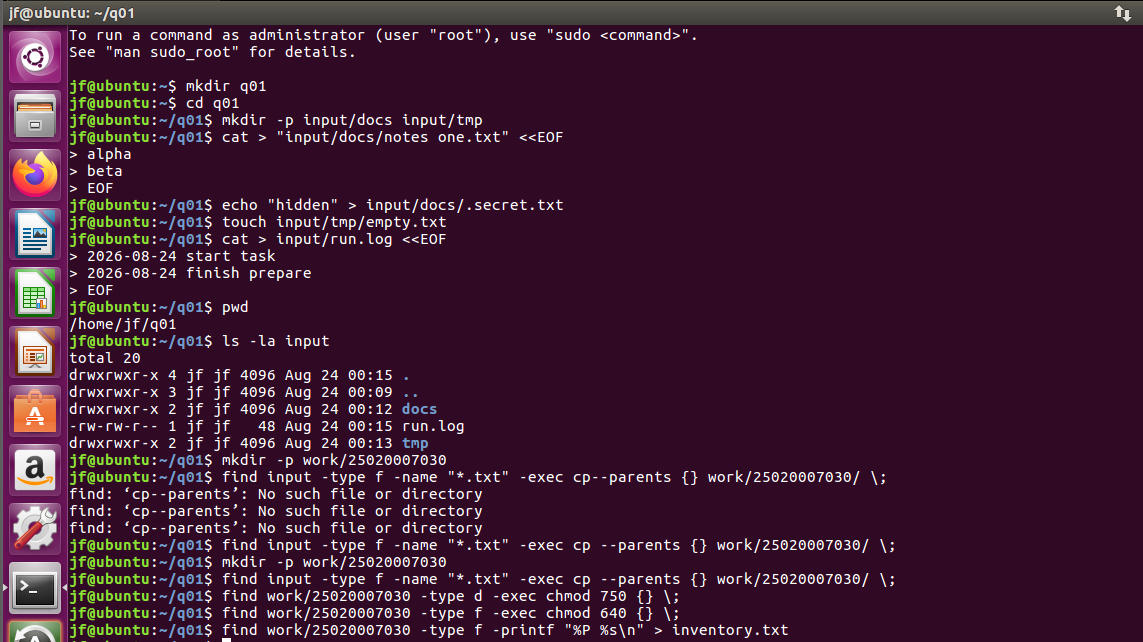
\includegraphics[width=0.9\textwidth]{fig_cls1_q01_process.png}
    \caption{第 1 题完整命令行作答过程}
    \label{fig:cls1_q01_process}
\end{figure}

\textbf{运行结果}

\begin{lstlisting}[caption={inventory.txt 内容（相对路径 + 字节数）}]
input/docs/.secret.txt 7
input/docs/notes one.txt 11
input/tmp/empty.txt 0
\end{lstlisting}

其中 \texttt{notes one.txt} 含文件名中的空格，在复制和统计时通过引号正确进行了处理；\texttt{.secret.txt} 为隐藏文件，\texttt{ls -a} 才能显示。inventory.txt 中给出了各文件的相对路径和实际字节数。

\begin{figure}[H]
    \centering
    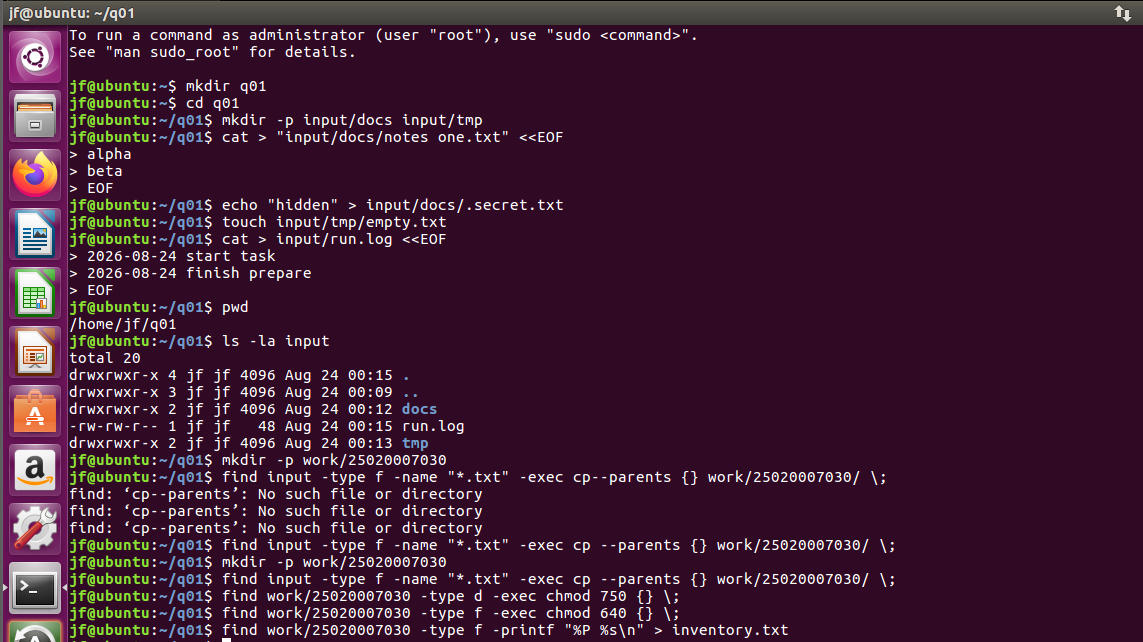
\includegraphics[width=0.9\textwidth]{fig_cls1_q01.png}
    \caption{第 1 题命令行操作与运行结果}
    \label{fig:cls1_q01}
\end{figure}

\textbf{助教检查结论}

\begin{tcolorbox}[colback=green!5, colframe=green!50!black, title={检查结果}]
    【待填写助教检查后的评价与打分，例如：】检查通过，助教评价：\underline{\hspace{6em}}，得分：\underline{\hspace{3em}}。
\end{tcolorbox}

% ----------------------------------------------------------------------------
% 1.2 第 2 题
% ----------------------------------------------------------------------------
\subsection{第 2 题：随机访问日志统计（Shell 管道与文本处理）}

\begin{tcolorbox}[colback=blue!5, colframe=blue!60!black, title={题目描述}]
    在 q02 中创建 \texttt{access.csv}，并使用给定数据完成日志统计：
    \begin{enumerate}
        \item 编写 \texttt{analyze.sh}，接收一个 CSV 文件路径；文件不存在时将错误写入 stderr 并返回非零退出码；
        \item 使用 Shell 管道以及 awk、sort、head 等工具，输出 HTTP 5xx 数量最多的前 2 个 path；按次数降序，次数相同时按 path 字典序；
        \item 输出全部数据行的平均 latency\_ms，保留两位小数；表头不得计入；
        \item 分别对 access.csv 和一个不存在的文件运行脚本；不得使用 Python、电子表格或手工统计。
    \end{enumerate}
\end{tcolorbox}

\textbf{作答过程与关键代码}

\begin{lstlisting}[language=bash, caption={analyze.sh 完整脚本}]
#!/bin/bash
csv_file="$1"
if [ ! -f "${csv_file}" ]; then
    echo "error: file ${csv_file} does not exist" >&2
    exit 1
fi
# 统计 5xx 最多的前 2 个 path：按次数降序、次数相同按字典序
awk -F',' 'NR>1 && $4 ~ /^5/ {print $3}' "${csv_file}" \
| sort | uniq -c | sort -k1,1nr -k2,2 | head -n 2
# 平均 latency_ms，保留两位小数（跳过表头）
awk -F',' 'NR>1 {sum += $5; cnt++} END {print sum, cnt}' "${csv_file}" \
| awk '{printf "%.2f\n", $1/$2}'
\end{lstlisting}

\begin{figure}[H]
    \centering
    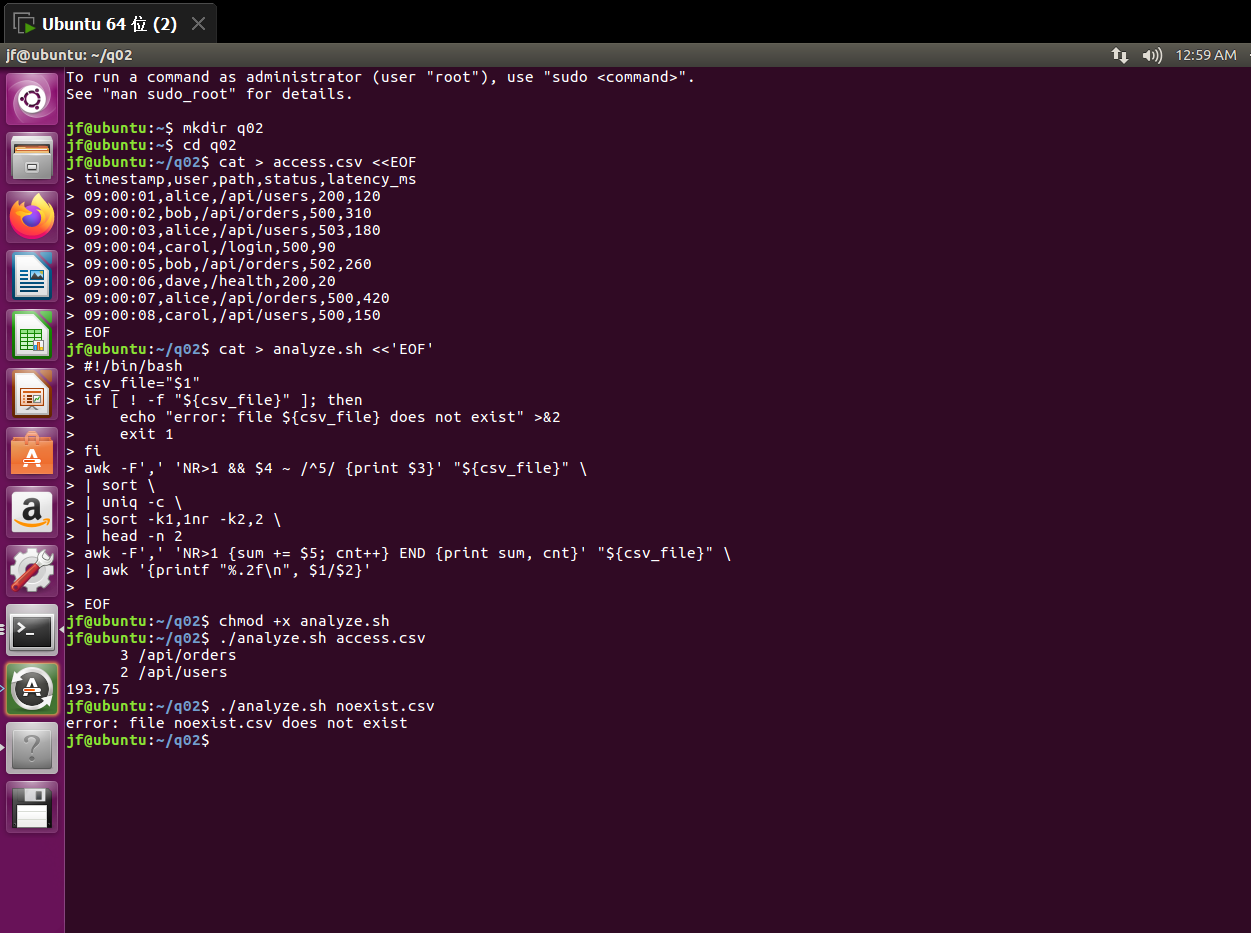
\includegraphics[width=0.9\textwidth]{fig_cls1_q02_process.png}
    \caption{第 2 题 access.csv 与 analyze.sh 的作答过程}
    \label{fig:cls1_q02_process}
\end{figure}

\textbf{运行结果}

对 \texttt{access.csv} 运行：
\begin{lstlisting}[language=bash, caption={对 access.csv 运行脚本}]
$ bash analyze.sh access.csv
      3 /api/orders
      2 /api/users
193.75
\end{lstlisting}

对不存在的文件运行：
\begin{lstlisting}[language=bash, caption={对不存在文件运行脚本}]
$ bash analyze.sh not_exist.csv
error: file not_exist.csv does not exist
$ echo $?
1
\end{lstlisting}

对不存在文件的错误信息写入了 stderr（\texttt{>\&2}），并通过 \texttt{exit 1} 返回非零退出码；5xx 状态行中 \texttt{/api/orders} 出现 3 次、\texttt{/api/users} 出现 2 次，为前 2 名；平均延迟 $(120+310+180+90+260+20+420+150)/8 = 193.75$。

\begin{figure}[H]
    \centering
    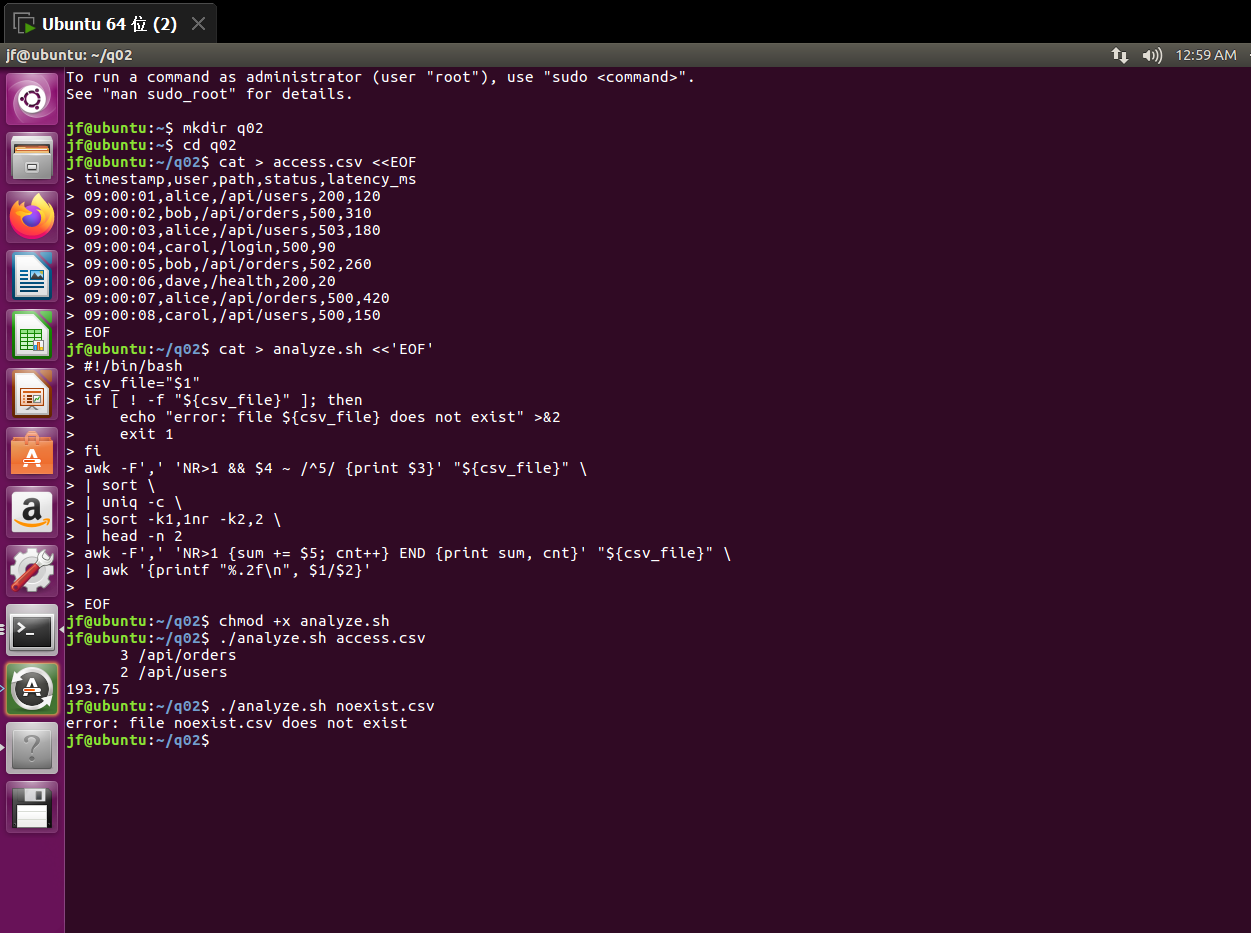
\includegraphics[width=0.9\textwidth]{fig_cls1_q02.png}
    \caption{第 2 题 access.csv、analyze.sh 及运行结果}
    \label{fig:cls1_q02}
\end{figure}

\textbf{助教检查结论}

\begin{tcolorbox}[colback=green!5, colframe=green!50!black, title={检查结果}]
    【待填写助教检查后的评价与打分，例如：】检查通过，助教评价：\underline{\hspace{6em}}，得分：\underline{\hspace{3em}}。
\end{tcolorbox}

% ----------------------------------------------------------------------------
% 1.3 第 3 题
% ----------------------------------------------------------------------------
\subsection{第 3 题：制造、解决并解释一次合并冲突（Git）}

\begin{tcolorbox}[colback=blue!5, colframe=blue!60!black, title={题目描述}]
    在 q03 中从零创建一个 Git 仓库，并主动制造、解决一次合并冲突：
    \begin{enumerate}
        \item 初始化仓库，在 main 创建 \texttt{config.txt}，内容为 \texttt{mode=normal}，并完成初始提交；
        \item 创建 \texttt{feature-a}，把内容改为 \texttt{mode=safe} 并提交；从初始 main 创建 \texttt{feature-b}，把内容改为 \texttt{mode=fast} 并提交；
        \item 回到 main，先合并 feature-a，再合并 feature-b；解决冲突时保留 \texttt{mode=safe}，并另加一行 \texttt{note=reviewed}；
        \item 确认工作区干净，运行 \texttt{git log --all --graph --decorate --oneline} 查看历史。
    \end{enumerate}
\end{tcolorbox}

\textbf{作答过程与关键代码}

\begin{lstlisting}[language=bash, caption={初始化并创建分支提交}]
cd q03 && git init
printf 'mode=normal\n' > config.txt
git add config.txt && git commit -m "init: mode=normal"
git switch -c feature-a
printf 'mode=safe\n' > config.txt
git add config.txt && git commit -m "feature-a: set mode=safe"
git switch master
git switch -c feature-b
printf 'mode=fast\n' > config.txt
git add config.txt && git commit -m "feature-b: set mode=fast"
\end{lstlisting}

\begin{lstlisting}[language=bash, caption={依次合并并解决冲突}]
git switch master
git merge feature-a          # 第一次合并：无冲突
git merge feature-b          # 第二次合并：产生冲突（同一行被不同修改）
# 编辑 config.txt，保留 mode=safe，另加一行 note=reviewed
git add config.txt
git commit -m "merge feature-b: resolve conflict, keep safe + note"
git status                   # 确认工作区干净
git log --all --graph --decorate --oneline
\end{lstlisting}

\begin{figure}[H]
    \centering
    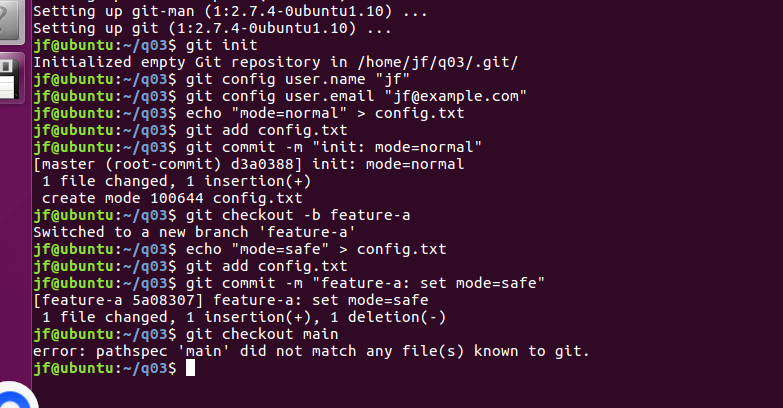
\includegraphics[width=0.9\textwidth]{fig_cls1_q03_process.png}
    \caption{第 3 题初始化仓库、创建分支的作答过程}
    \label{fig:cls1_q03_process}
\end{figure}

\textbf{运行结果}

解决冲突后的 \texttt{config.txt}：
\begin{lstlisting}[caption={config.txt 最终内容}]
mode=safe
note=reviewed
\end{lstlisting}

\texttt{git log --all --graph --decorate --oneline} 输出：
\begin{lstlisting}[caption={提交历史图（merge-log.txt）}]
* 25c1246 (HEAD -> master) merge feature-b: resolve conflict, keep safe + note
*   8ab4aeb merge feature-b: resolve conflict, keep safe + note
|\
| * aa6594e (feature-b) feature-b: set mode=fast
* | 5a08307 (feature-a) feature-a: set mode=safe
|/
* d3a0388 init: mode=normal
\end{lstlisting}

冲突产生的原因是 feature-a 与 feature-b 都修改了 \texttt{config.txt} 的同一行（\texttt{mode=}），Git 无法自动判断保留哪一个，于是产生了冲突标记；手工编辑时保留了 \texttt{mode=safe} 并增加 \texttt{note=reviewed}，完成合并后工作区干净。

\begin{figure}[H]
    \centering
    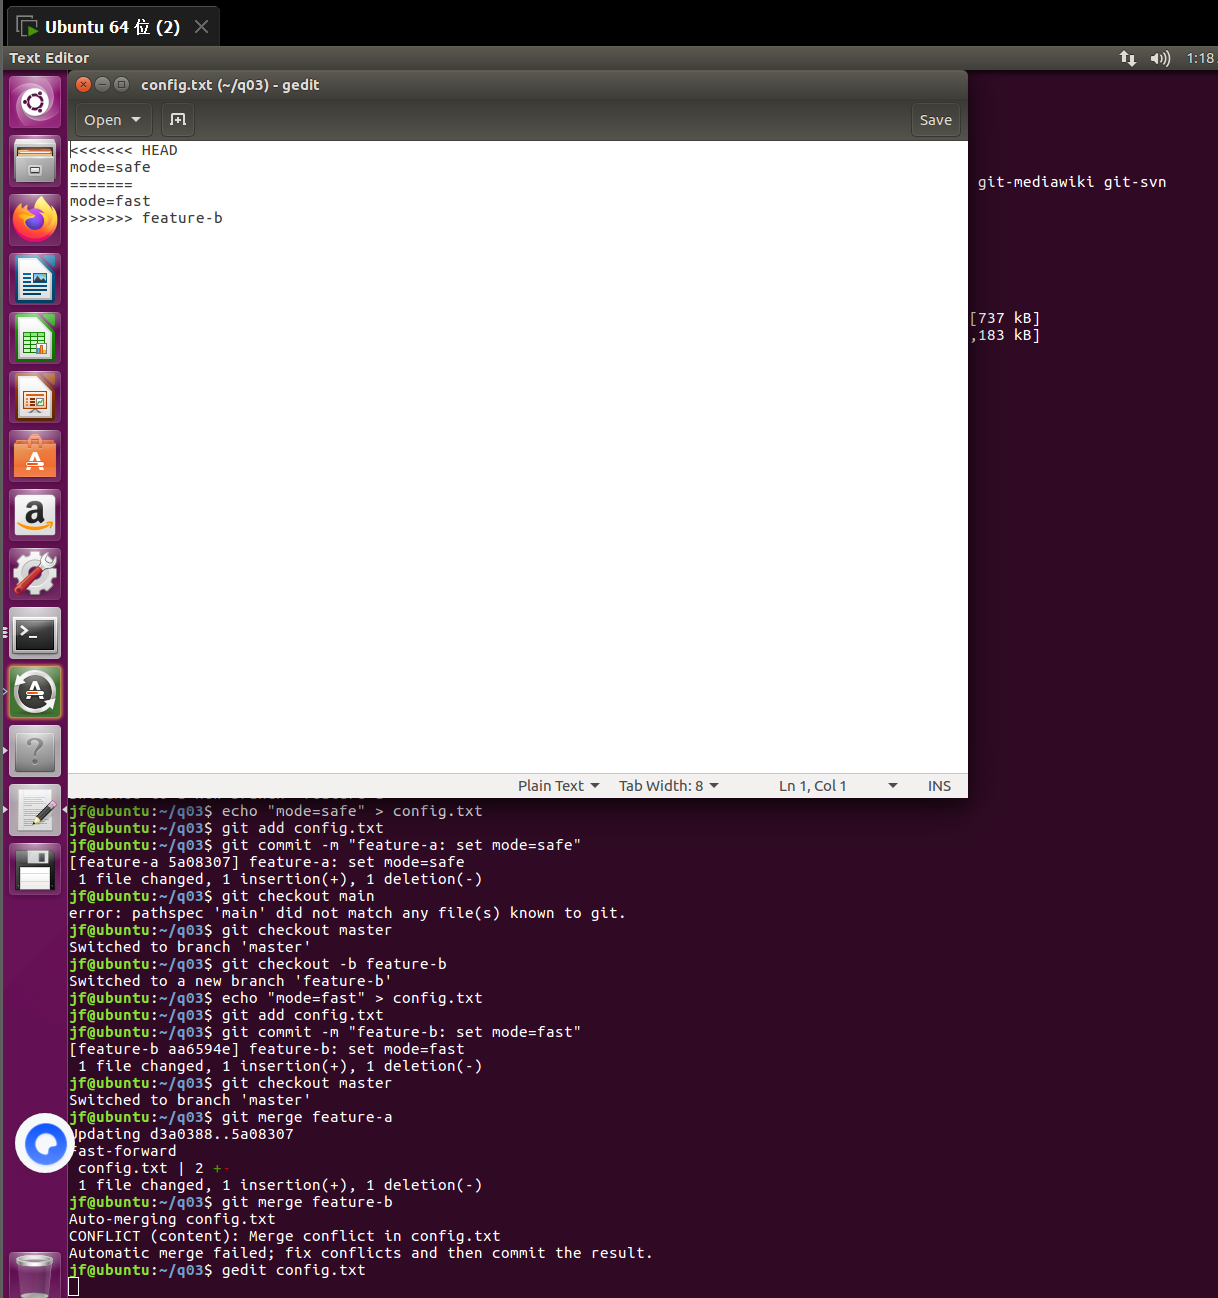
\includegraphics[width=0.9\textwidth]{fig_cls1_q03_conflict.png}
    \caption{第 3 题 gedit 中看到的冲突标记及产生冲突的过程}
    \label{fig:cls1_q03_conflict}
\end{figure}

\begin{figure}[H]
    \centering
    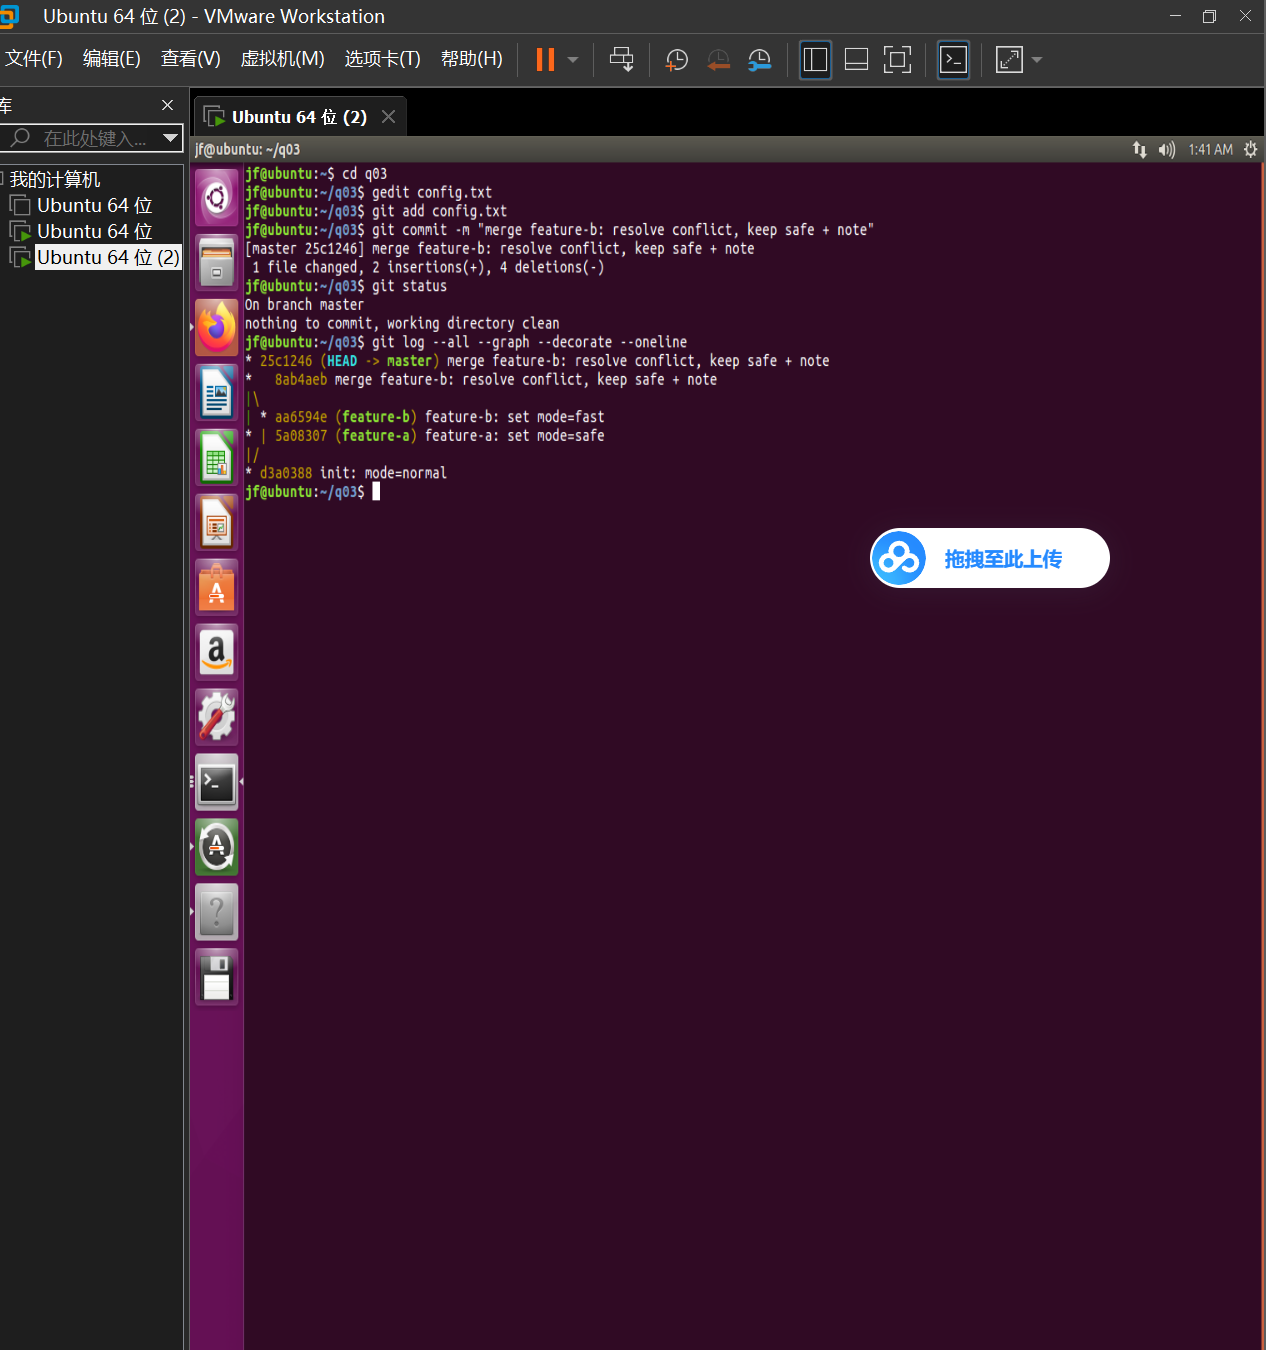
\includegraphics[width=0.9\textwidth]{fig_cls1_q03_resolved.png}
    \caption{第 3 题解决冲突并提交后的提交历史图}
    \label{fig:cls1_q03_resolved}
\end{figure}

\textbf{助教检查结论}

\begin{tcolorbox}[colback=green!5, colframe=green!50!black, title={检查结果}]
    【待填写助教检查后的评价与打分，例如：】检查通过，助教评价：\underline{\hspace{6em}}，得分：\underline{\hspace{3em}}。
\end{tcolorbox}

% ----------------------------------------------------------------------------
% 1.4 第 4 题
% ----------------------------------------------------------------------------
\subsection{第 4 题：修复并构建一页技术说明（LaTeX 文档编辑）}

\begin{tcolorbox}[colback=blue!5, colframe=blue!60!black, title={题目描述}]
    将给定模板保存为 \texttt{q04/report.tex}，补全内容并从命令行构建 PDF：
    \begin{enumerate}
        \item 加入一个带编号和 label 的公式，并在正文中使用 ref 或 eqref 引用；
        \item 加入一个 2 行 2 列表格，设置 caption 和 label，并在正文中引用该表；
        \item 使用 \texttt{latexmk -pdf -halt-on-error} 或 \texttt{tectonic} 生成 \texttt{report.pdf}；
        \item 确认 PDF 能打开，且交叉引用不显示 ``??''。
    \end{enumerate}
\end{tcolorbox}

\textbf{作答过程与关键代码}

\begin{lstlisting}[language=tex, caption={report.tex 补全后的关键内容}]
\documentclass{article}
\usepackage{amsmath}
\begin{document}
\title{Tool Report}
\author{jf-25020007030}
\maketitle

\section{Result}
The calculation formula is shown in Equation~\eqref{eq:test_formula}

\begin{equation}
E=mc^2
\label{eq:test_formula}
\end{equation}

Table~\ref{tab:data_table}
\begin{table}[h]
\centering
\caption{Experimental comparison data}
\label{tab:data_table}
\begin{tabular}{|c|c|}
\hline
A & B \\
\hline
10 & 20 \\
\hline
30 & 40 \\
\hline
\end{tabular}
\end{table}

Equation~\eqref{eq:test_formula} is mass-energy relation;
Table~\ref{tab:data_table} records sample measurement
\end{document}
\end{lstlisting}

\begin{figure}[H]
    \centering
    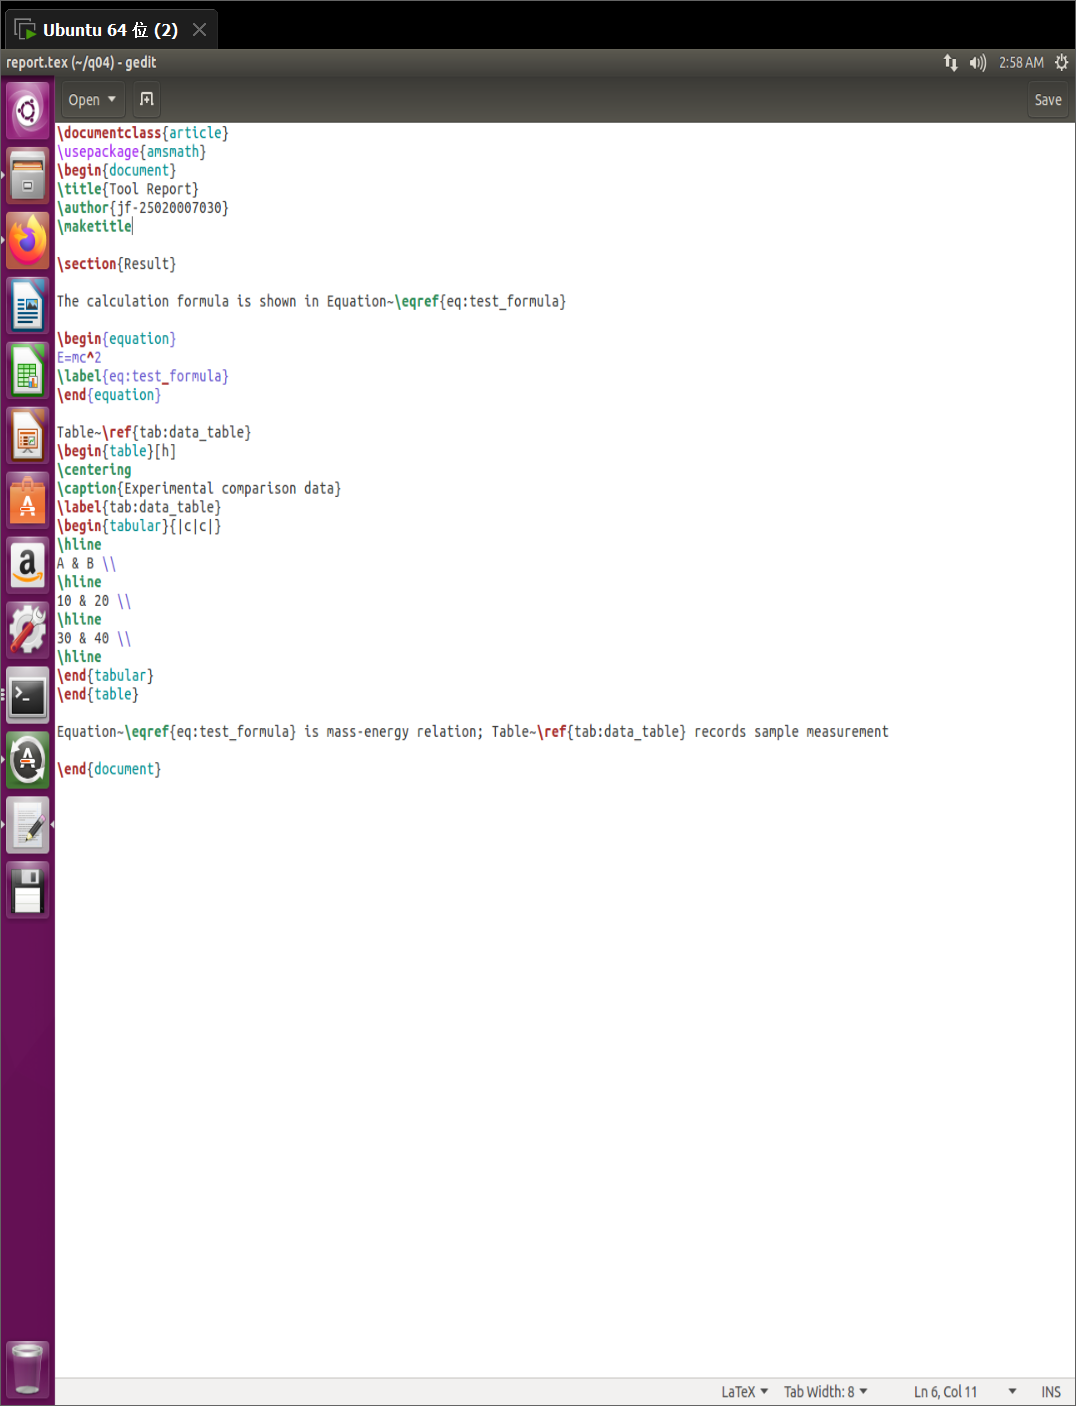
\includegraphics[width=0.9\textwidth]{fig_cls1_q04_process.png}
    \caption{第 4 题用 gedit 编辑 report.tex 的作答过程}
    \label{fig:cls1_q04_process}
\end{figure}

\textbf{运行结果}

使用 \texttt{latexmk -pdf -halt-on-error report.tex} 编译成功，生成了 \texttt{report.pdf}。PDF 可正常打开，正文中公式引用显示为 ``(1)''、表格引用显示为 ``1''，交叉引用不再出现 ``??''，说明 \texttt{\\label} 与 \texttt{\\eqref}/\\texttt{\\ref} 对应关系正确。

\begin{figure}[H]
    \centering
    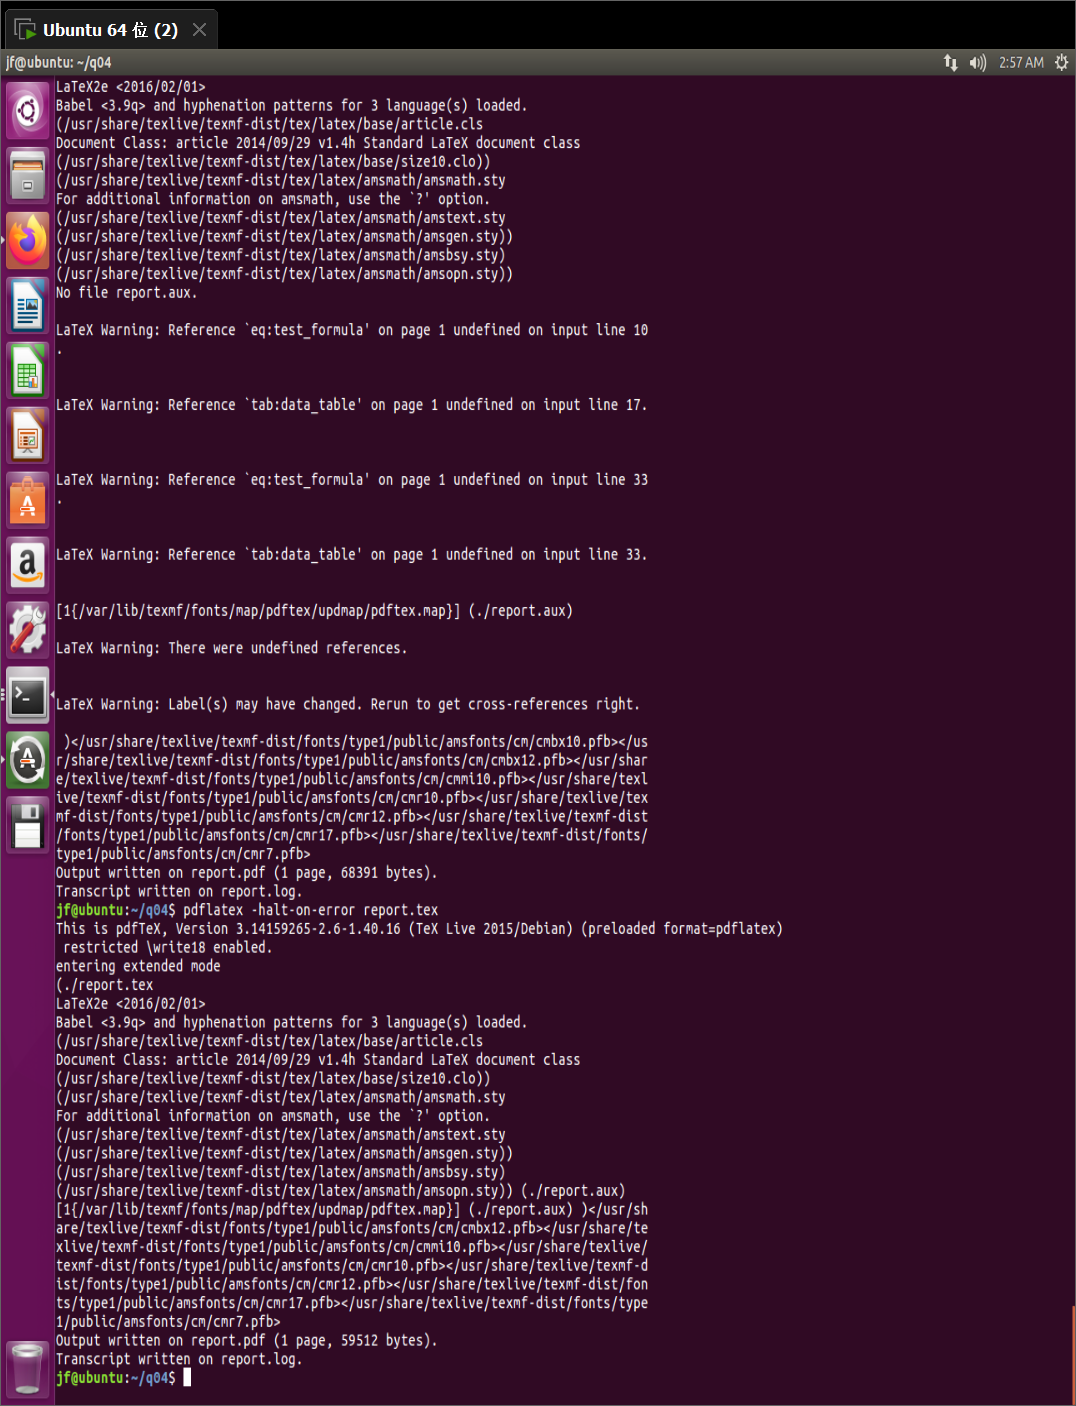
\includegraphics[width=0.9\textwidth]{fig_cls1_q04_compile.png}
    \caption{第 4 题 pdflatex 编译 report.tex 生成 report.pdf}
    \label{fig:cls1_q04_compile}
\end{figure}

\begin{figure}[H]
    \centering
    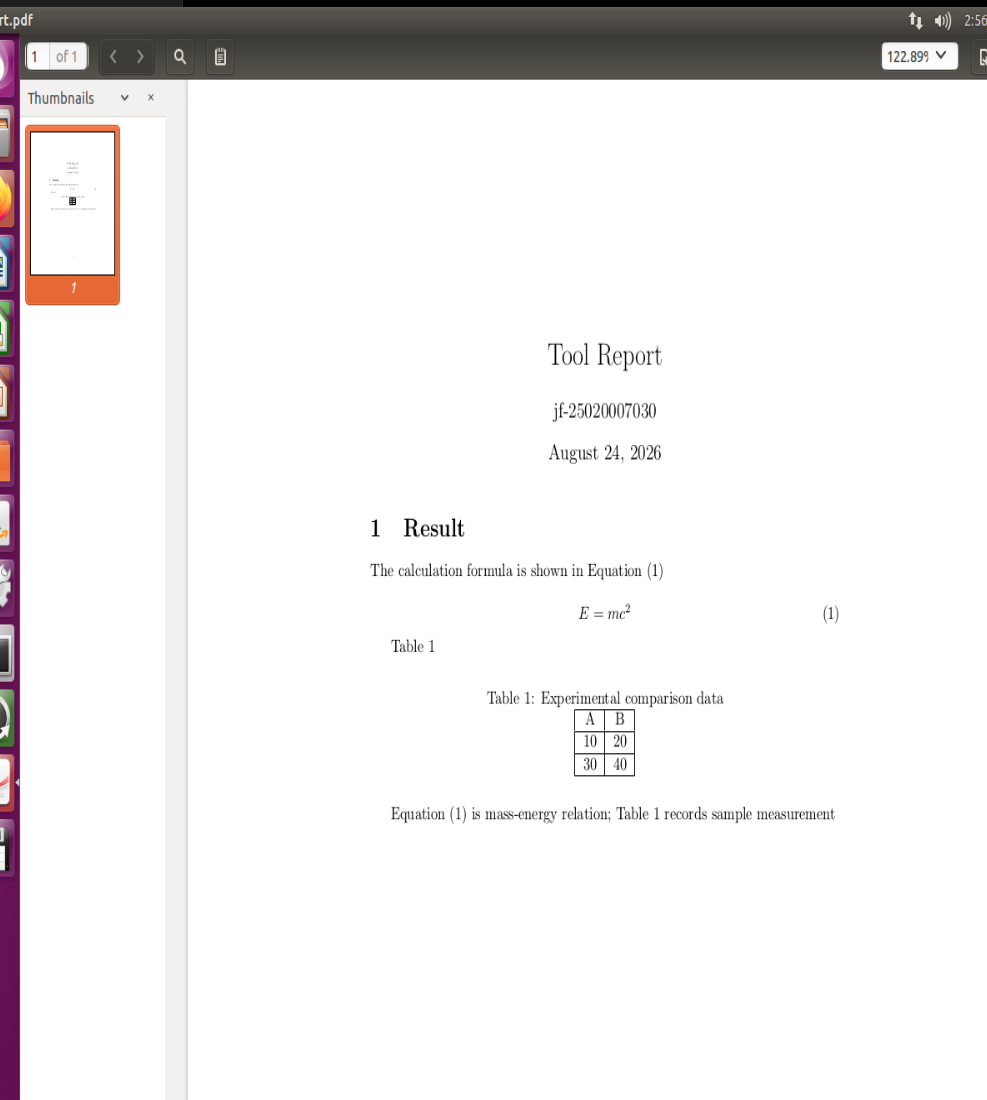
\includegraphics[width=0.75\textwidth]{fig_cls1_q04_pdf.png}
    \caption{第 4 题编译生成的 report.pdf 成品}
    \label{fig:cls1_q04_pdf}
\end{figure}

\textbf{助教检查结论}

\begin{tcolorbox}[colback=green!5, colframe=green!50!black, title={检查结果}]
    【待填写助教检查后的评价与打分，例如：】检查通过，助教评价：\underline{\hspace{6em}}，得分：\underline{\hspace{3em}}。
\end{tcolorbox}

% ============================================================================
% 2. 课后练习内容和结果
% ============================================================================
\section{课后练习内容和结果}

课后共完成 11 个实例练习，按「题目—作答—结果」记录如下。按照课程要求，练习内容均已分步提交到个人 GitHub 仓库，并禁止单次全量提交。

\subsection{Shell 基础与文件系统练习}

\subsubsection{第 2 题：ls 的 -l 选项（flag）作用是什么？}

\textbf{题目}：运行 \texttt{ls -l /} 并观察输出，每一行最前面的 10 个字符分别代表什么？

\begin{figure}[H]
    \centering
    
\includegraphics[width=0.9\textwidth]{fig_hw2_question.png}
    \caption{第 2 题题目截图}
    \label{fig:hw2_question}
\end{figure}

\textbf{作答}：\texttt{-l} 选项以长格式输出文件信息。每行最前面 10 个字符含义如下（以 \texttt{-rw-r--r--} 为例）：

\begin{table}[H]
    \centering
    \renewcommand{\arraystretch}{1.3}
    \begin{tabular}{p{2.2cm}p{12.0cm}}
        \toprule
        第 1 个字符 & 文件类型：\texttt{-} 普通文件、\texttt{d} 目录、\texttt{l} 符号链接、\texttt{b}/\texttt{c} 块/字符设备等 \\
        \midrule
        第 2--4 个字符 & 属主（user）的读、写、执行权限（r/w/x，无权限为 -） \\
        第 5--7 个字符 & 属组（group）的读、写、执行权限 \\
        第 8--10 个字符 & 其他用户（other）的读、写、执行权限 \\
        \bottomrule
    \end{tabular}
    \caption{ls -l 前 10 个字符含义}
\end{table}

\textbf{结果}：运行 \texttt{ls -l /} 后，每行形如 \texttt{drwxr-xr-x 1 root root 4096 ...}，其中 \texttt{drwxr-xr-x} 表明该目录属主可读可写可执行、属组和其他用户可读可执行。可通过 \texttt{man ls} 查看帮助确认。

\begin{figure}[H]
    \centering
    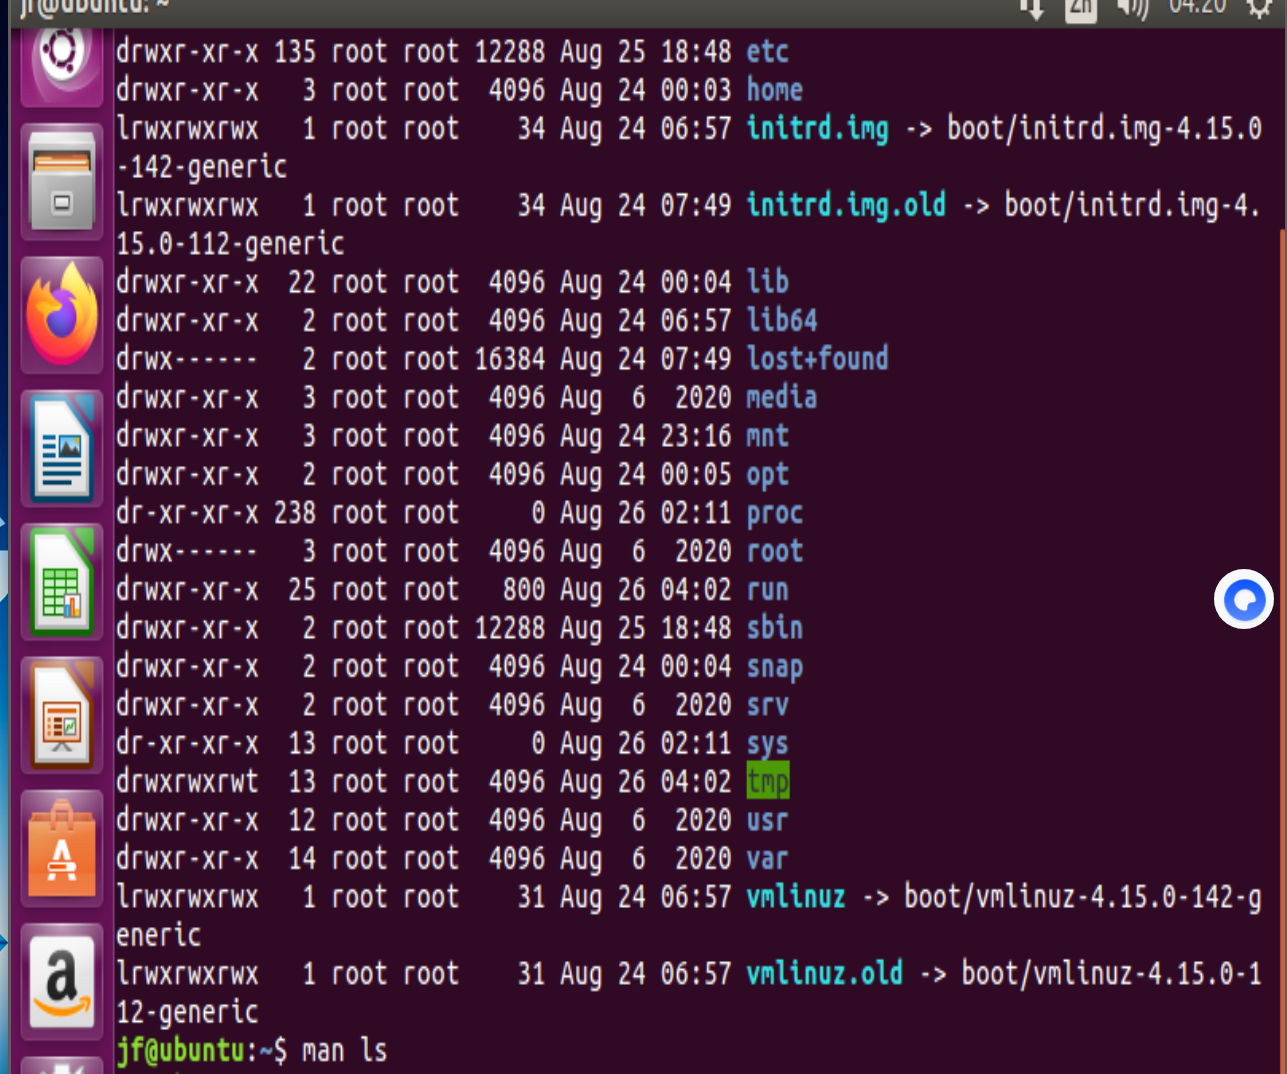
\includegraphics[width=0.9\textwidth]{fig_q2_ls_l.png}
    \caption{运行 ls -l / 的结果}
    \label{fig:q2_ls_l}
\end{figure}


\subsubsection{第 5 题：Shell 标准流与重定向}

\textbf{题目}：Shell 有三条标准流 stdin（0）、stdout（1）、stderr（2）。运行 \texttt{ls /nonexistent /tmp}，把 stdout 和 stderr 分别重定向到两个文件。你将如何把两者都重定向到同一个文件？

\begin{figure}[H]
    \centering
    
\includegraphics[width=0.9\textwidth]{fig_hw5_question.png}
    \caption{第 5 题题目截图}
    \label{fig:hw5_question}
\end{figure}

\textbf{作答}：
\begin{lstlisting}[language=bash, caption={分别重定向 stdout 与 stderr}]
ls /nonexistent /tmp > out.txt 2> err.txt
# 将 stdout 与 stderr 都重定向到同一个文件
ls /nonexistent /tmp > all.txt 2>&1
\end{lstlisting}

\textbf{结果}：
\begin{itemize}
    \item \texttt{out.txt}：只包含 /tmp 的正常列表输出（stdout）；
    \item \texttt{err.txt}：只包含 \texttt{ls: cannot access '/nonexistent': No such file or directory}（stderr）；
    \item \texttt{all.txt}：使用 \texttt{2>\&1} 将 stderr 合并到 stdout 后，两类内容写入同一文件。
\end{itemize}

\begin{figure}[H]
    \centering
    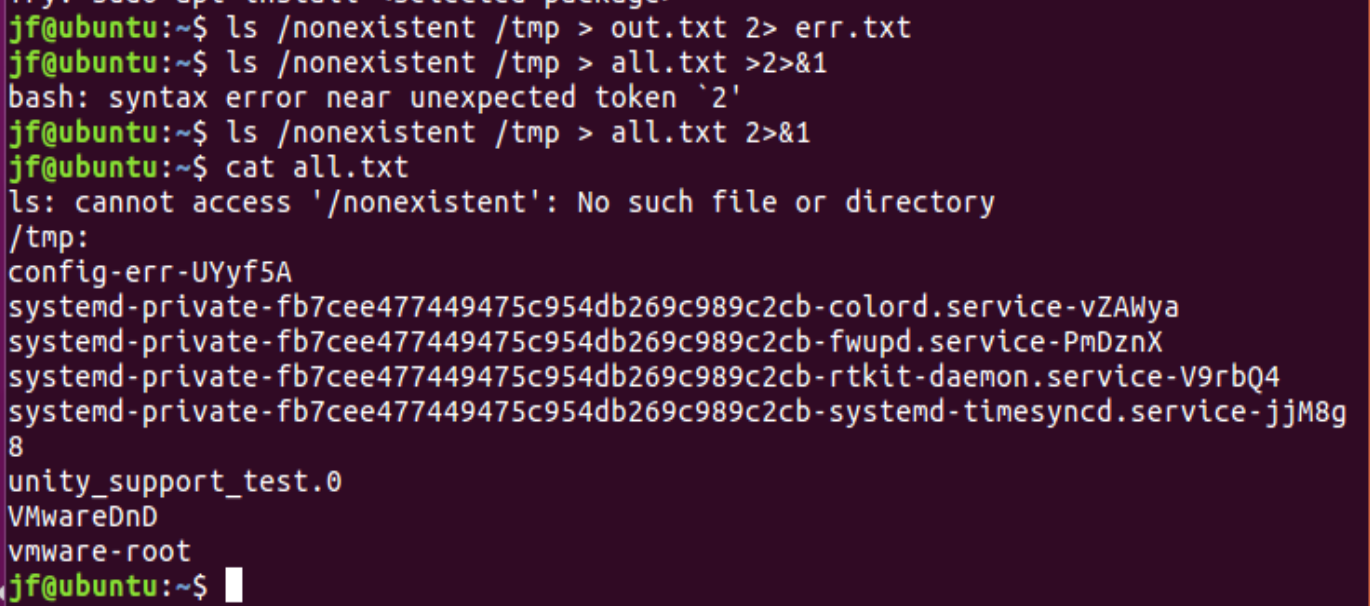
\includegraphics[width=0.9\textwidth]{fig_q5_redirect.png}
    \caption{标准流重定向的运行结果}
    \label{fig:q5_redirect}
\end{figure}

\subsubsection{第 8 题：检查文件是否存在的脚本}

\textbf{题目}：写一个脚本，接收文件名参数（\$1），用 \texttt{test -f} 或 \texttt{[ -f ... ]} 检查该文件是否存在，并根据结果输出不同提示。

\begin{figure}[H]
    \centering
    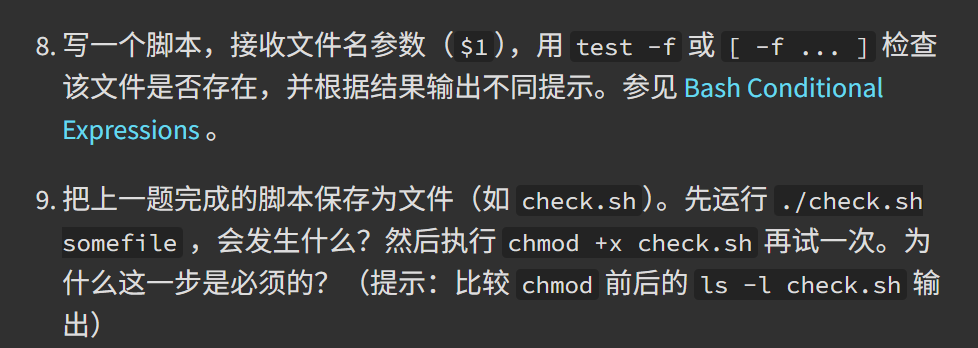
\includegraphics[width=0.9\textwidth]{fig_hw8_question.png}
    \caption{第 8、9 题题目截图}
    \label{fig:hw8_question}
\end{figure}

\textbf{作答}：
\begin{lstlisting}[language=bash, caption={check.sh}]
#!/bin/bash
if [ -f "$1" ]; then
    echo "file $1 exist"
else
    echo "file $1 no exist"
fi
\end{lstlisting}

\textbf{结果}：
\begin{lstlisting}[language=bash, caption={运行结果}]
$ bash check.sh somefile
file somefile exist
$ bash check.sh not_exist
file not_exist no exist
\end{lstlisting}

\begin{figure}[H]
    \centering
    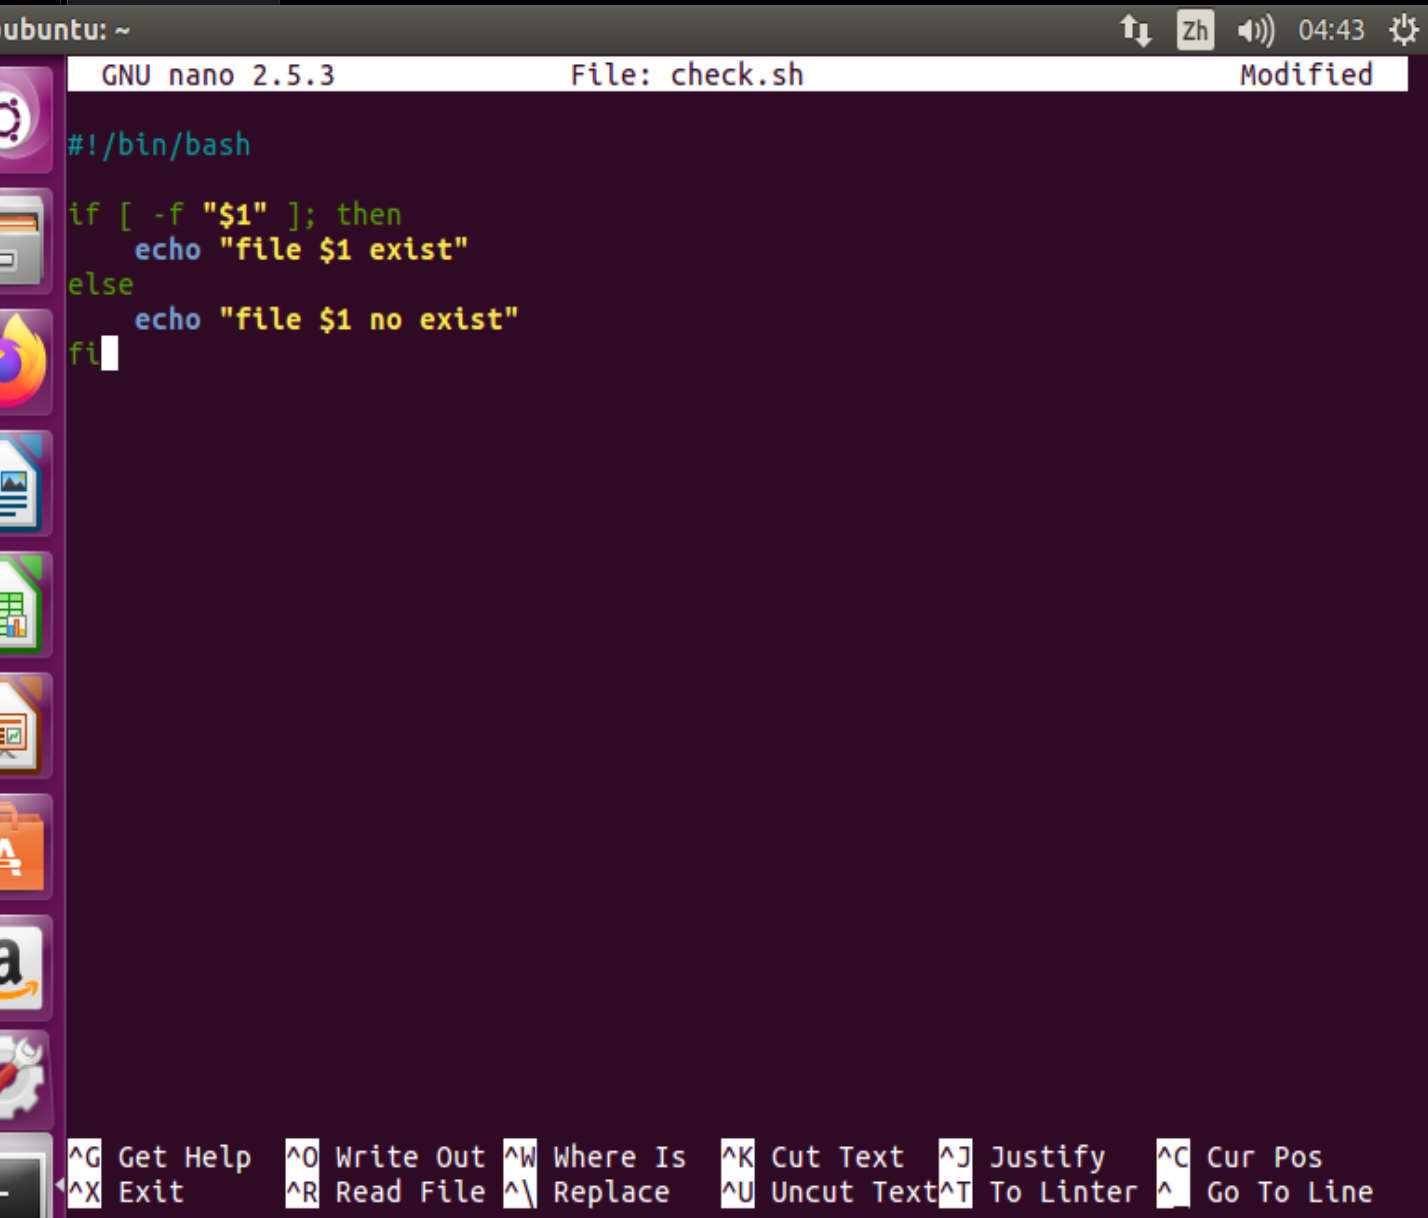
\includegraphics[width=0.85\textwidth]{fig_q8_check_sh_nano.png}
    \caption{用 nano 编写 check.sh 脚本}
    \label{fig:q8_check_sh}
\end{figure}

\subsubsection{第 9 题：为脚本添加可执行权限（chmod）}

\textbf{题目}：把上一题脚本保存为 \texttt{check.sh}。先运行 \texttt{./check.sh somefile}，会发生什么？然后执行 \texttt{chmod +x check.sh} 再试一次。为什么这一步是必须的？

\textbf{作答}：直接运行 \texttt{./check.sh} 时，由于文件没有可执行权限，Shell 会报 \texttt{Permission denied}；执行 \texttt{chmod +x check.sh} 后再运行则正常。权限是操作系统对文件执行的访问控制，只有具备 \texttt{x}（execute）权限的文件才能被直接执行；\texttt{chmod +x} 即为属主、属组和其他用户添加执行权限。

\textbf{结果}：
\begin{lstlisting}[language=bash, caption={chmod 前后对比}]
$ ls -l check.sh          # 修改前
-rw-r--r-- 1 jf jf ... check.sh
$ ./check.sh somefile
bash: ./check.sh: Permission denied
$ chmod +x check.sh
$ ls -l check.sh          # 修改后，属主出现 x 权限
-rwxr-xr-x 1 jf jf ... check.sh
$ ./check.sh somefile
file somefile exist
\end{lstlisting}

\begin{figure}[H]
    \centering
    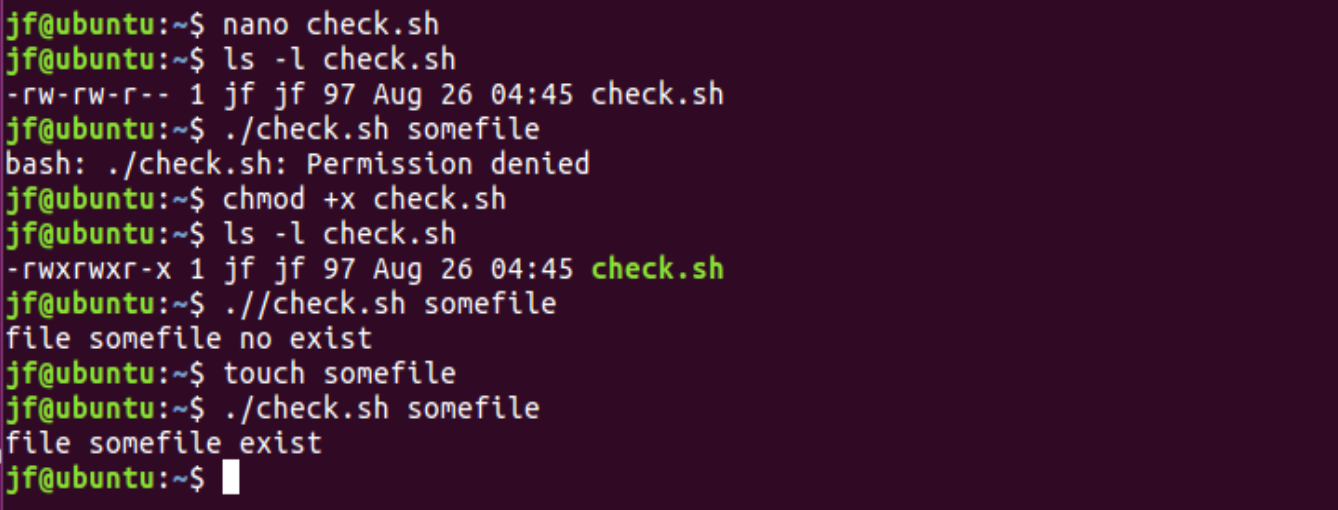
\includegraphics[width=0.9\textwidth]{fig_q9_chmod.png}
    \caption{chmod +x 前后对比及运行结果}
    \label{fig:q9_chmod}
\end{figure}

\subsubsection{第 10 题：set -x 选项的作用}

\textbf{题目}：在脚本的 set 选项里加入 \texttt{-x} 会发生什么？写个简单脚本试试并观察输出。

\begin{figure}[H]
    \centering
    
\includegraphics[width=0.9\textwidth]{fig_hw10_question.png}
    \caption{第 10 题题目截图}
    \label{fig:hw10_question}
\end{figure}

\textbf{作答}：\texttt{set -x} 开启命令跟踪（xtrace），脚本执行时会把每条将要执行的命令（展开后的形式，前缀 \texttt{+}）打印到 stderr，便于调试。

\begin{lstlisting}[language=bash, caption={测试 set -x 的脚本}]
#!/bin/bash
set -x
echo "hello"
ls /nonexistent
\end{lstlisting}

\textbf{结果}：运行后输出类似：
\begin{lstlisting}[caption={set -x 输出}]
+ echo hello
hello
+ ls /nonexistent
ls: cannot access '/nonexistent': No such file or directory
\end{lstlisting}

可以看到每条命令都被打印出来（前面带 \texttt{+}），方便定位脚本执行到哪一步出错。参见 Bash 的 The Set Builtin。

\begin{figure}[H]
    \centering
    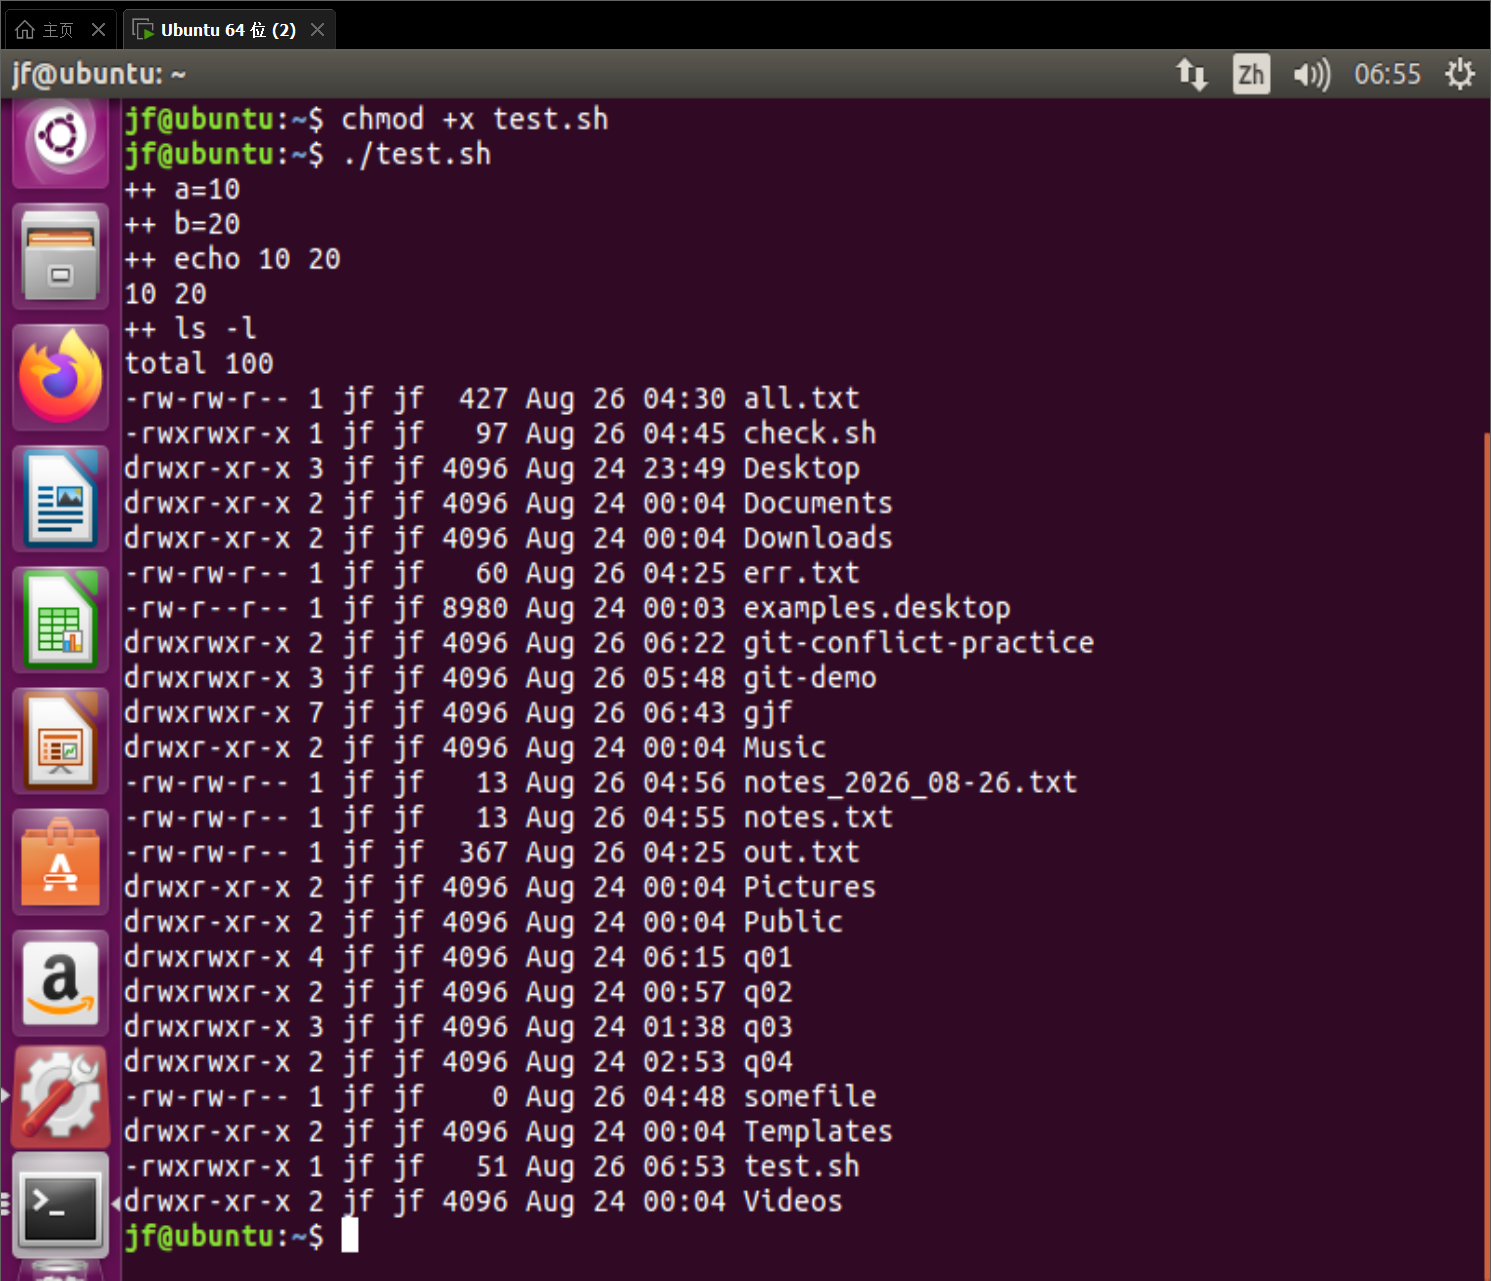
\includegraphics[width=0.9\textwidth]{fig_q10_set_x.png}
    \caption{运行带 set -x 的脚本，逐条追踪命令}
    \label{fig:q10_set_x}
\end{figure}

\subsubsection{第 11 题：带当天日期的备份文件名}

\textbf{题目}：写一条命令，把文件复制为带当天日期的备份文件名（例如 \texttt{notes.txt} $\rightarrow$ \texttt{notes\_2026-01-12.txt}）。

\begin{figure}[H]
    \centering
    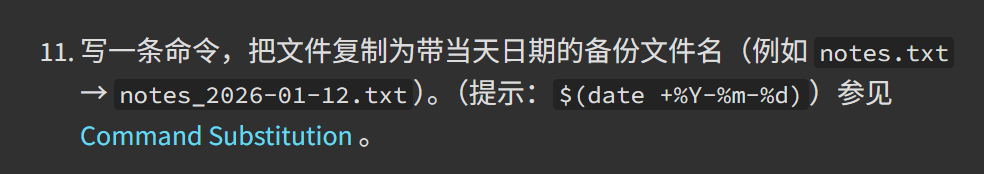
\includegraphics[width=0.9\textwidth]{fig_hw11_question.png}
    \caption{第 11 题题目截图}
    \label{fig:hw11_question}
\end{figure}

\textbf{作答}：使用命令替换 \texttt{\$(date +\%Y-\%m-\%d)} 生成当天日期：
\begin{lstlisting}[language=bash, caption={带日期备份命令}]
cp notes.txt "notes_$(date +%Y-%m-%d).txt"
\end{lstlisting}

\textbf{结果}：2026 年 8 月 26 日执行后生成 \texttt{notes\_2026\_08-26.txt}，内容与 \texttt{notes.txt} 一致（\texttt{test content}）。

\begin{figure}[H]
    \centering
    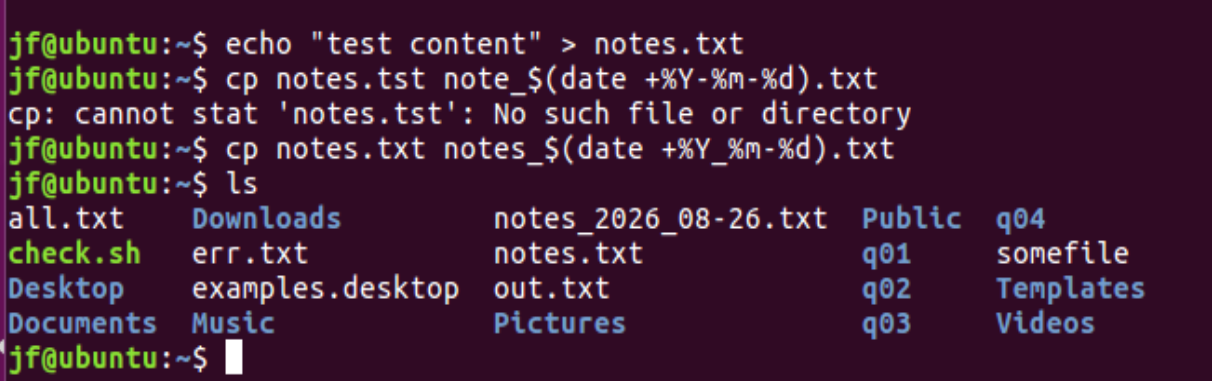
\includegraphics[width=0.9\textwidth]{fig_q11_date_backup.png}
    \caption{带当天日期的备份文件名运行结果}
    \label{fig:q11_date_backup}
\end{figure}

\subsection{Git 版本控制练习}

\subsubsection{第 3 题：从 Git 历史中删除误提交的文件}

\textbf{题目}：学习 Git 时常见的错误是把不应由 Git 管理的大文件或敏感信息提交进去。尝试添加一个文件、做几次提交，然后从历史记录中删除该文件（而不仅是删掉最新提交）。

\begin{figure}[H]
    \centering
    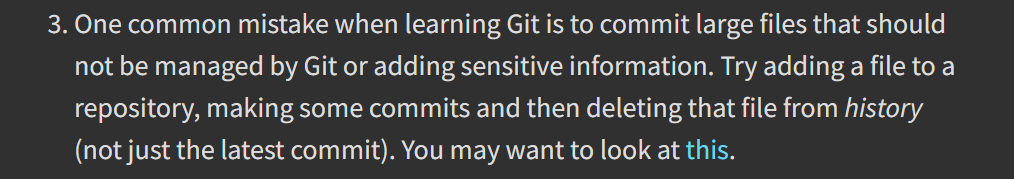
\includegraphics[width=0.9\textwidth]{fig_git3_question.png}
    \caption{Git 第 3 题题目截图}
    \label{fig:git3_question}
\end{figure}

\textbf{作答}：将文件加入仓库并提交后，若需从历史中彻底删除，可使用 \texttt{git filter-branch} 或 \texttt{git rebase -i} 改写历史：
\begin{lstlisting}[language=bash, caption={从历史删除文件}]
git filter-branch --force --index-filter \
  'git rm --cached --ignore-unmatch secret.txt' --prune-empty -- --all
# 清理残留对象
git for-each-ref --format='%(refname)' refs/original/ | xargs -n1 git update-ref -d
git reflog expire --expire=now --all && git gc --prune=now --aggressive
\end{lstlisting}

\textbf{结果}：改写后的提交历史中不再包含该文件；此操作通常用于删除敏感信息或超大文件，但会改写历史哈希，仅适用于尚未推送或可接受强制推送的场景。

\begin{figure}[H]
    \centering
    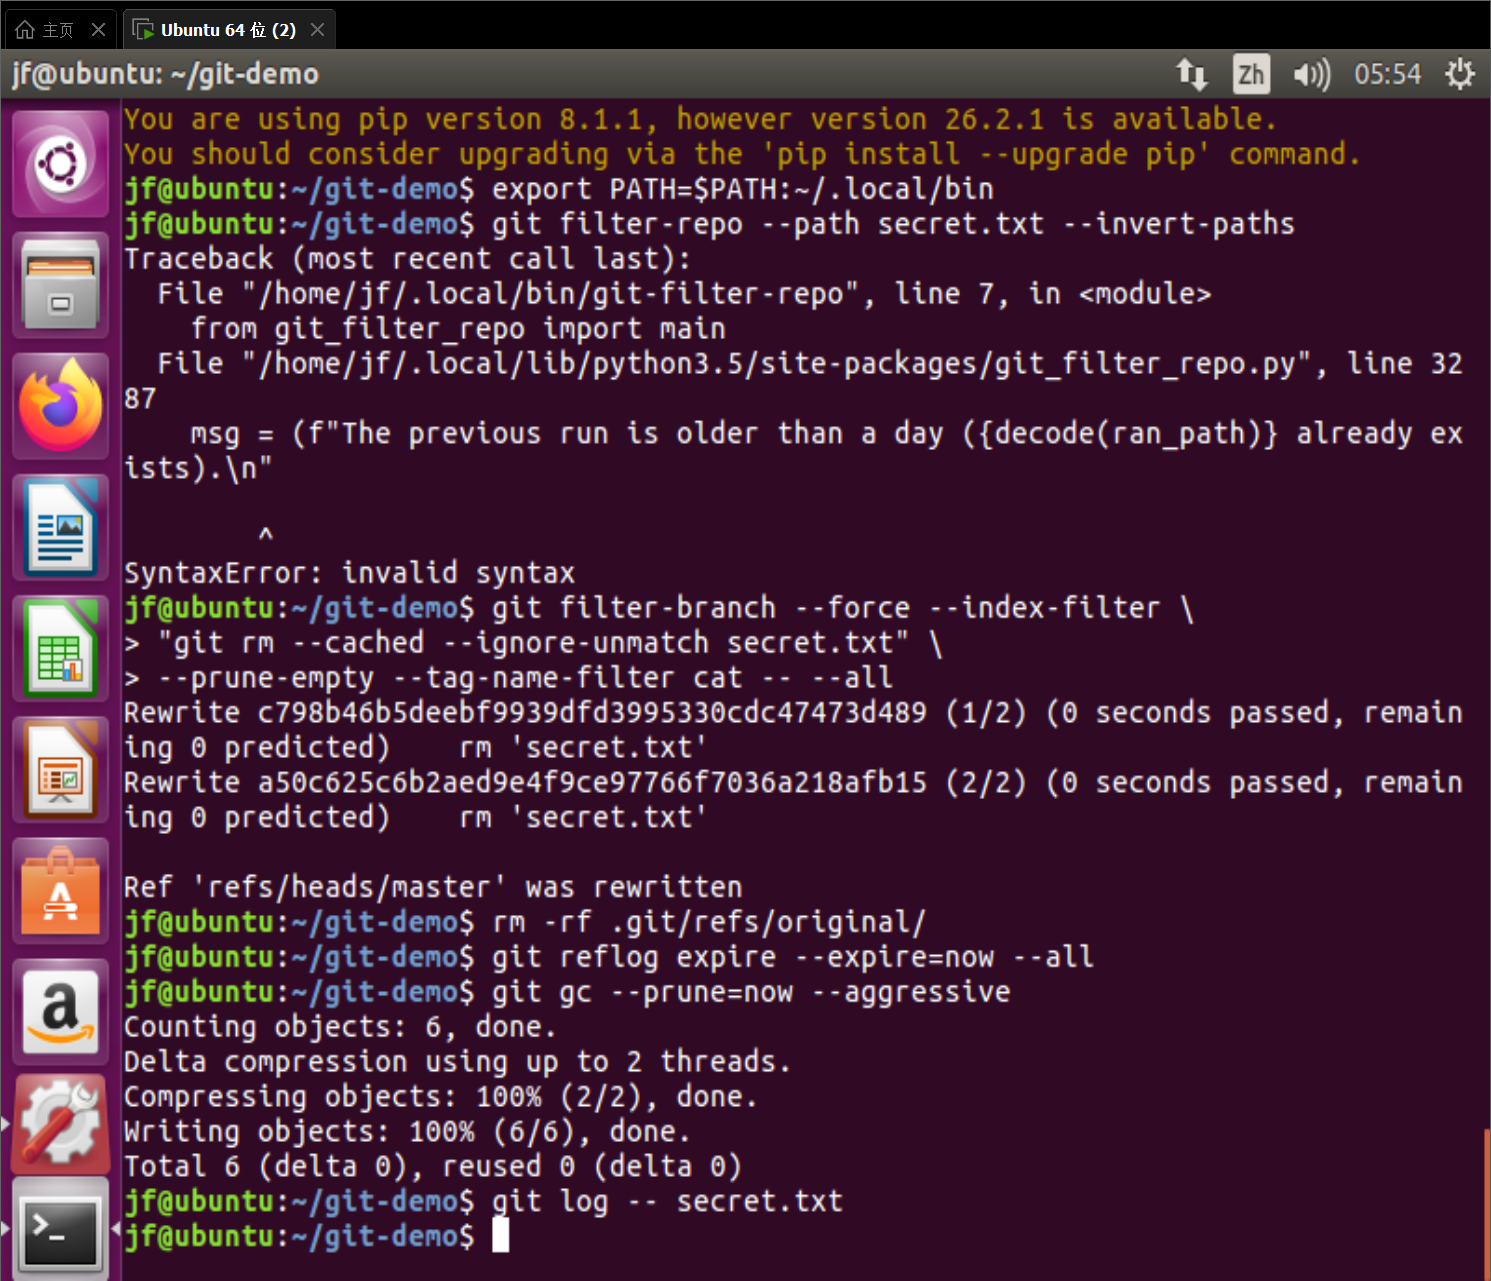
\includegraphics[width=0.9\textwidth]{fig_git3_filter_branch.png}
    \caption{用 git filter-branch 从历史中删除 secret.txt}
    \label{fig:git3_filter_branch}
\end{figure}

\subsubsection{第 4 题：git stash 暂存未完成的工作}

\textbf{题目}：从 GitHub 克隆某个仓库，修改其中一个已有文件。做 \texttt{git stash} 会发生什么？运行 \texttt{git log --all --oneline} 会看到什么？运行 \texttt{git stash pop} 来撤销刚才的操作。这个操作在什么场景下有用？

\begin{figure}[H]
    \centering
    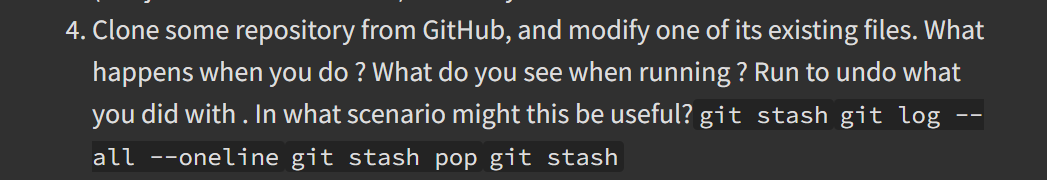
\includegraphics[width=0.9\textwidth]{fig_git4_question.png}
    \caption{Git 第 4 题题目截图}
    \label{fig:git4_question}
\end{figure}

\textbf{作答}：\texttt{git stash} 会把工作区的未提交修改临时保存起来，使工作区恢复干净；\texttt{git log --all --oneline} 会看到当前分支及 stash 创建的相关提交（stash 也会记录一条 WIP 提交）；\texttt{git stash pop} 把暂存的修改恢复到工作区。

\textbf{结果}：该操作在需要临时切换分支、却不想丢弃或提交当前半成品修改时非常有用，例如接到紧急任务需切走时，可先 \texttt{git stash}，处理完再 \texttt{git stash pop} 恢复。

\begin{figure}[H]
    \centering
    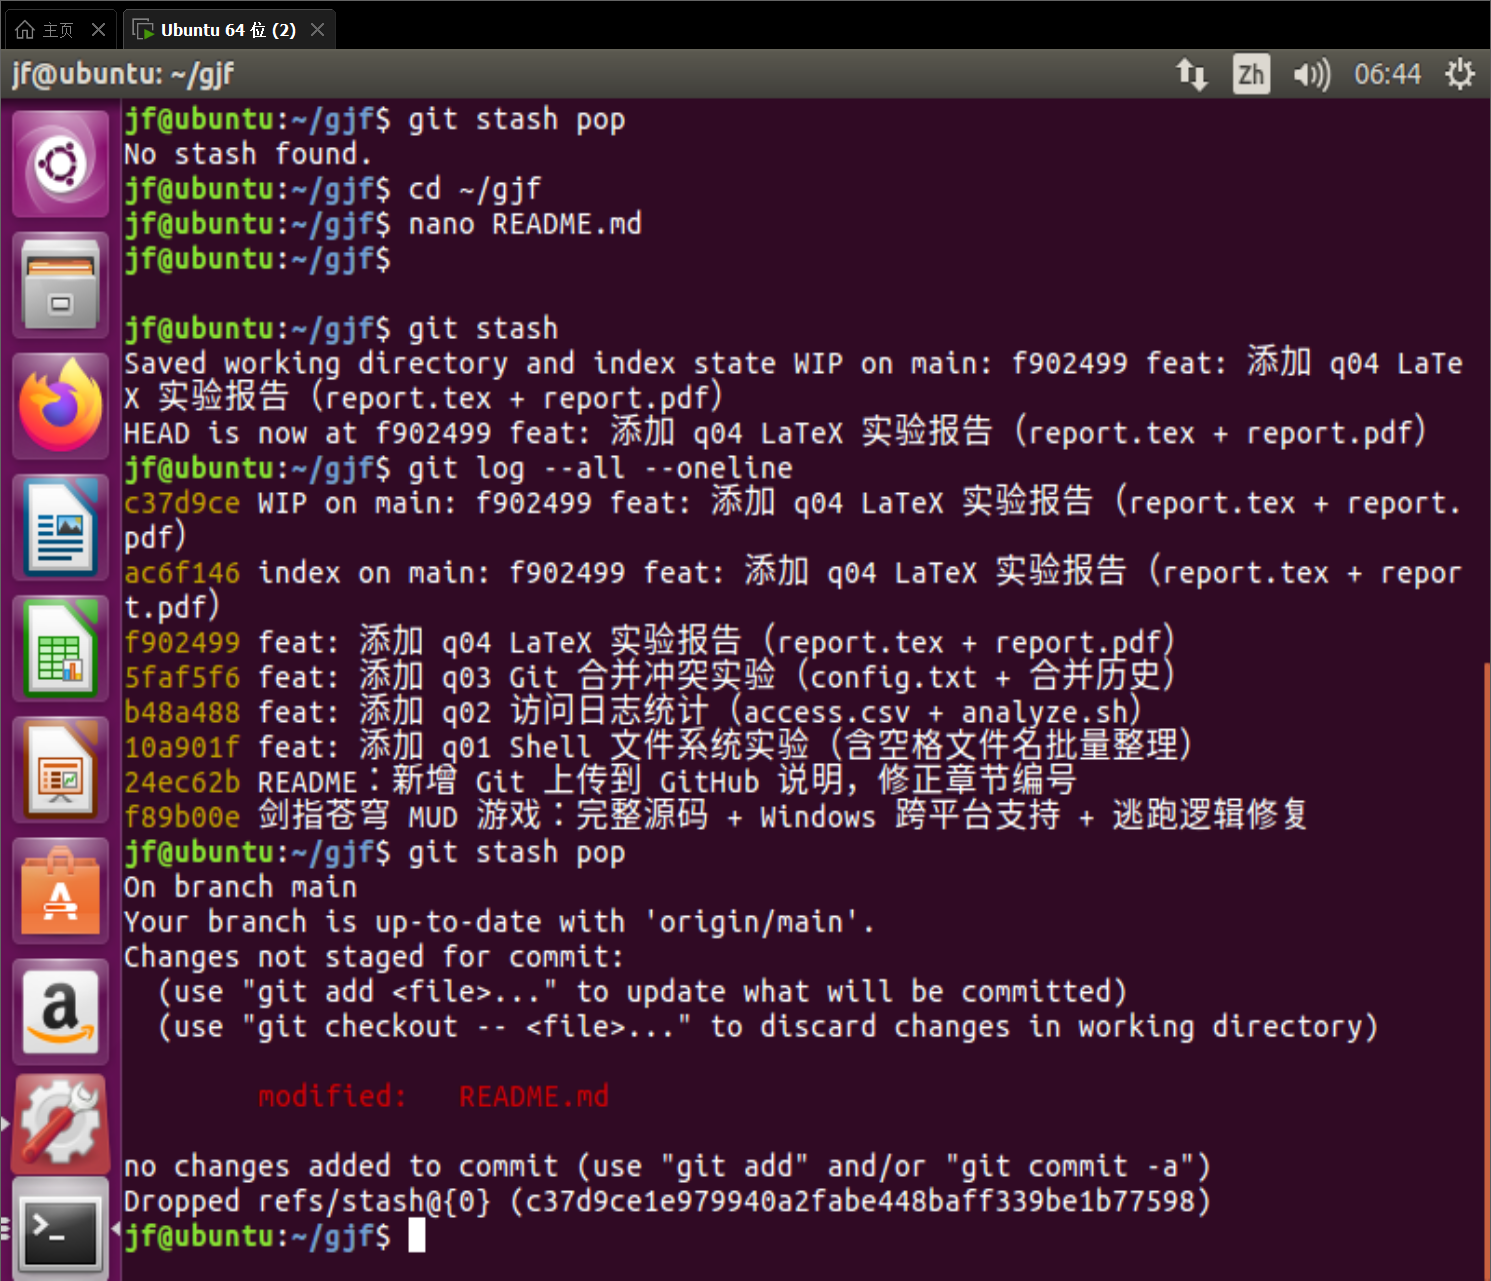
\includegraphics[width=0.9\textwidth]{fig_git4_stash.png}
    \caption{git stash 与 git stash pop 的完整过程}
    \label{fig:git4_stash}
\end{figure}

\subsubsection{第 5 题：为 git log 配置别名}

\textbf{题目}：Git 提供配置文件 \texttt{\~/.gitconfig}。创建一个别名，使运行 \texttt{git graph} 时得到 \texttt{git log --all --graph --decorate --oneline} 的输出。

\begin{figure}[H]
    \centering
    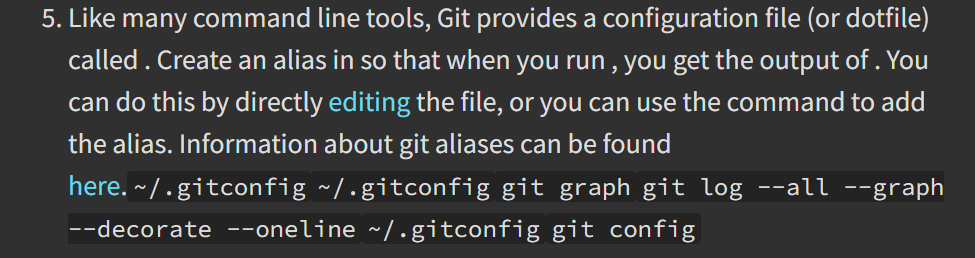
\includegraphics[width=0.9\textwidth]{fig_git5_question.png}
    \caption{Git 第 5 题题目截图}
    \label{fig:git5_question}
\end{figure}

\textbf{作答}：
\begin{lstlisting}[language=bash, caption={配置 git 别名}]
git config --global alias.graph "log --all --graph --decorate --oneline"
# 之后即可用
git graph
\end{lstlisting}

\textbf{结果}：配置写入 \texttt{\~/.gitconfig} 的 \texttt{[alias]} 段。之后 \texttt{git graph} 即可输出图形化的完整提交历史。

\begin{figure}[H]
    \centering
    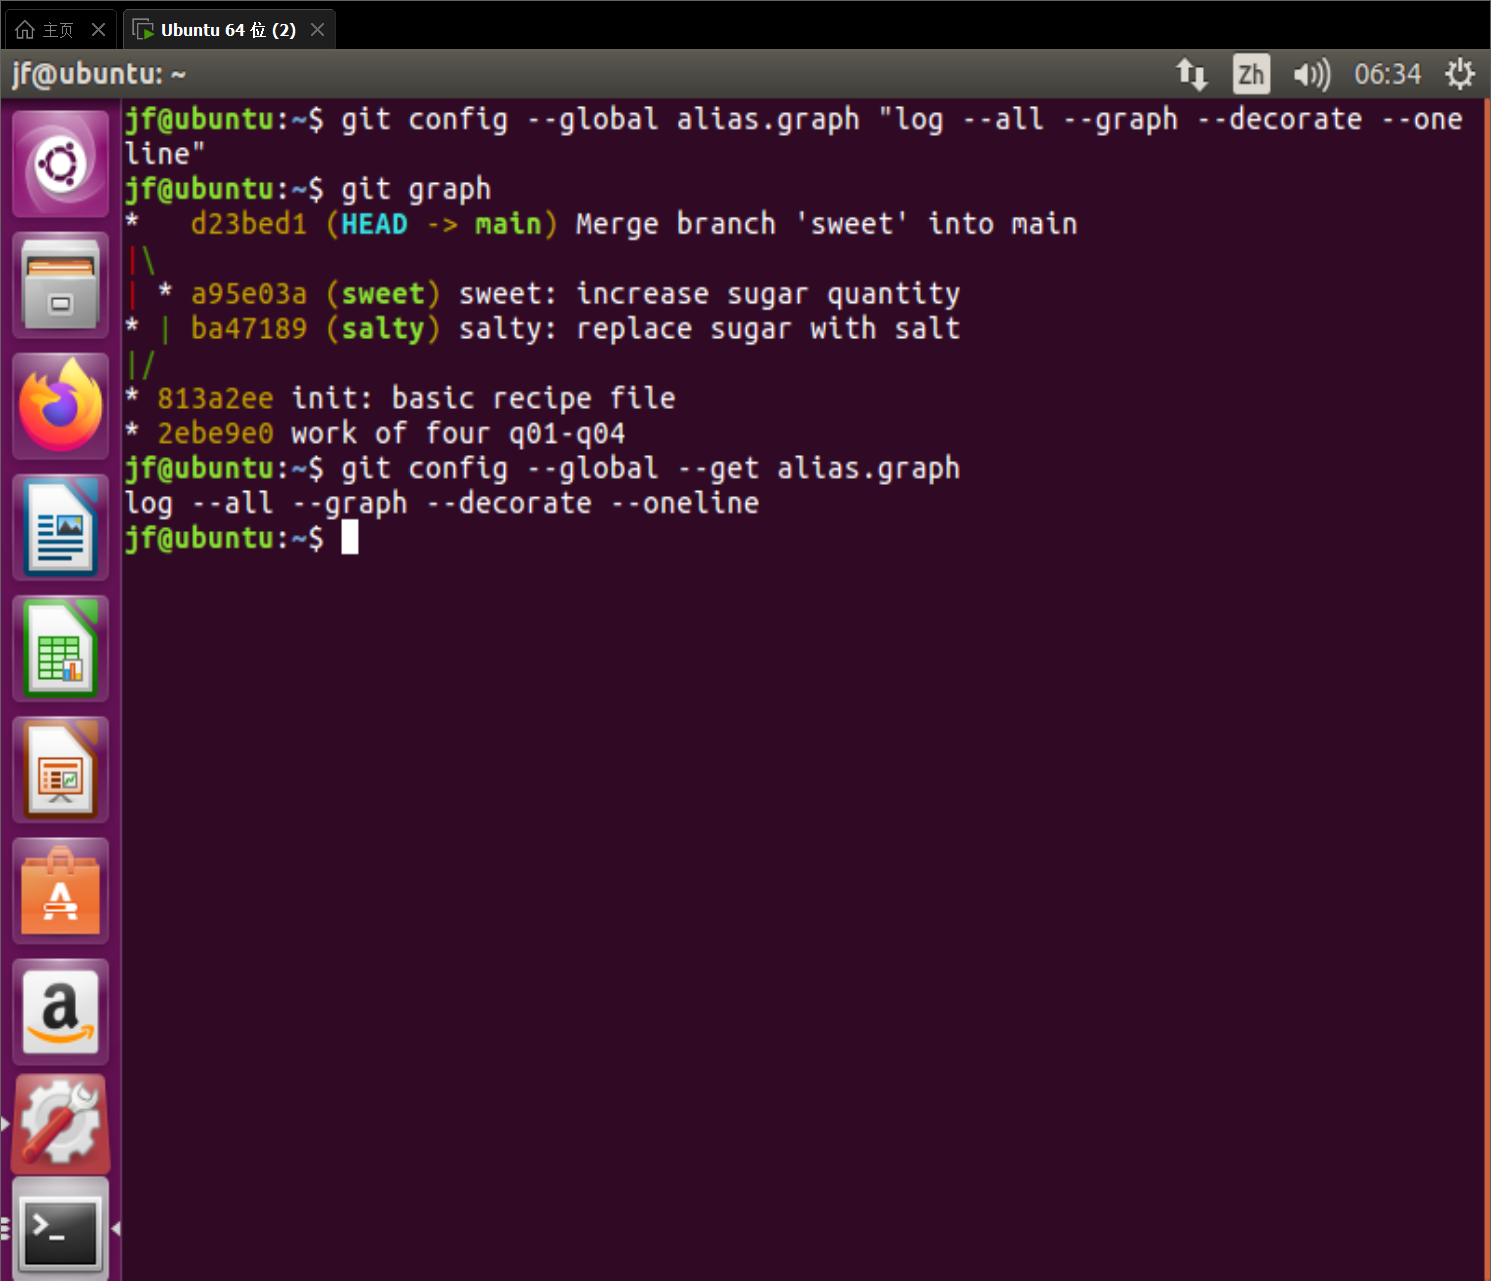
\includegraphics[width=0.9\textwidth]{fig_git5_alias.png}
    \caption{配置 git graph 别名并运行}
    \label{fig:git5_alias}
\end{figure}

\subsubsection{第 6 题：配置全局 gitignore}

\textbf{题目}：通过 \texttt{git config --global core.excludesfile} 指定全局忽略文件路径，并手动创建该文件，忽略操作系统或编辑器产生的临时文件。

\begin{figure}[H]
    \centering
    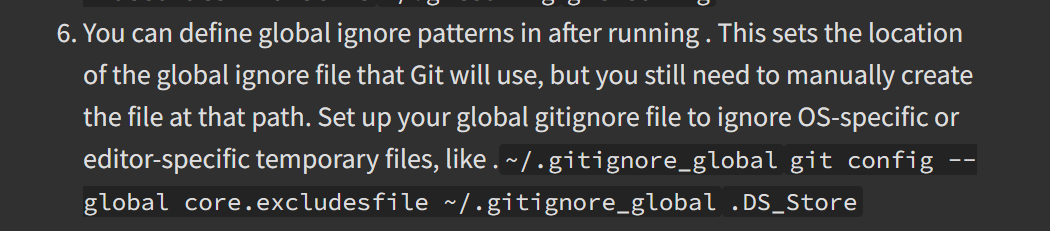
\includegraphics[width=0.9\textwidth]{fig_git6_question.png}
    \caption{Git 第 6 题题目截图}
    \label{fig:git6_question}
\end{figure}

\textbf{作答}：
\begin{lstlisting}[language=bash, caption={配置全局忽略文件}]
touch ~/.gitignore_global
git config --global core.excludesfile ~/.gitignore_global
echo '.DS_Store' >> ~/.gitignore_global
echo 'Thumbs.db' >> ~/.gitignore_global
\end{lstlisting}

\textbf{结果}：全局忽略文件生效，所有仓库都会忽略 macOS/Windows 系统临时文件（如 \texttt{.DS\_Store}、\texttt{Thumbs.db}），避免误提交。

\begin{figure}[H]
    \centering
    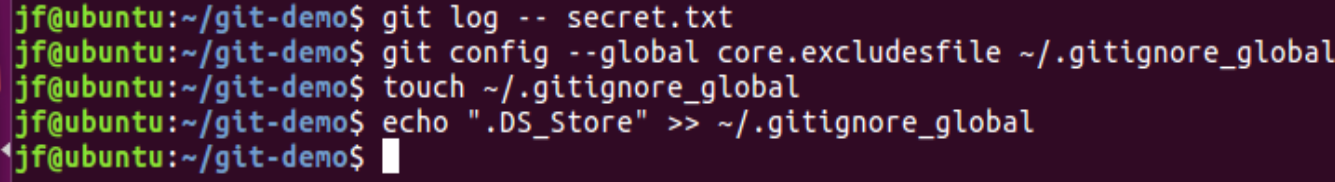
\includegraphics[width=0.9\textwidth]{fig_git6_gitignore.png}
    \caption{配置全局 gitignore 文件}
    \label{fig:git6_gitignore}
\end{figure}

\subsubsection{第 8 题：模拟协作场景解决合并冲突}

\textbf{题目}：创建一个仓库和 \texttt{recipe.txt}（如一个简单的菜谱），提交后创建 \texttt{salty} 和 \texttt{sweet} 两个分支；分别在两个分支修改同一行并提交；切回 master 依次合并两个分支触发冲突，查看冲突标记含义，编辑文件解决冲突并完成合并，最后用 \texttt{git log --graph --oneline} 查看合并历史。

\begin{figure}[H]
    \centering
    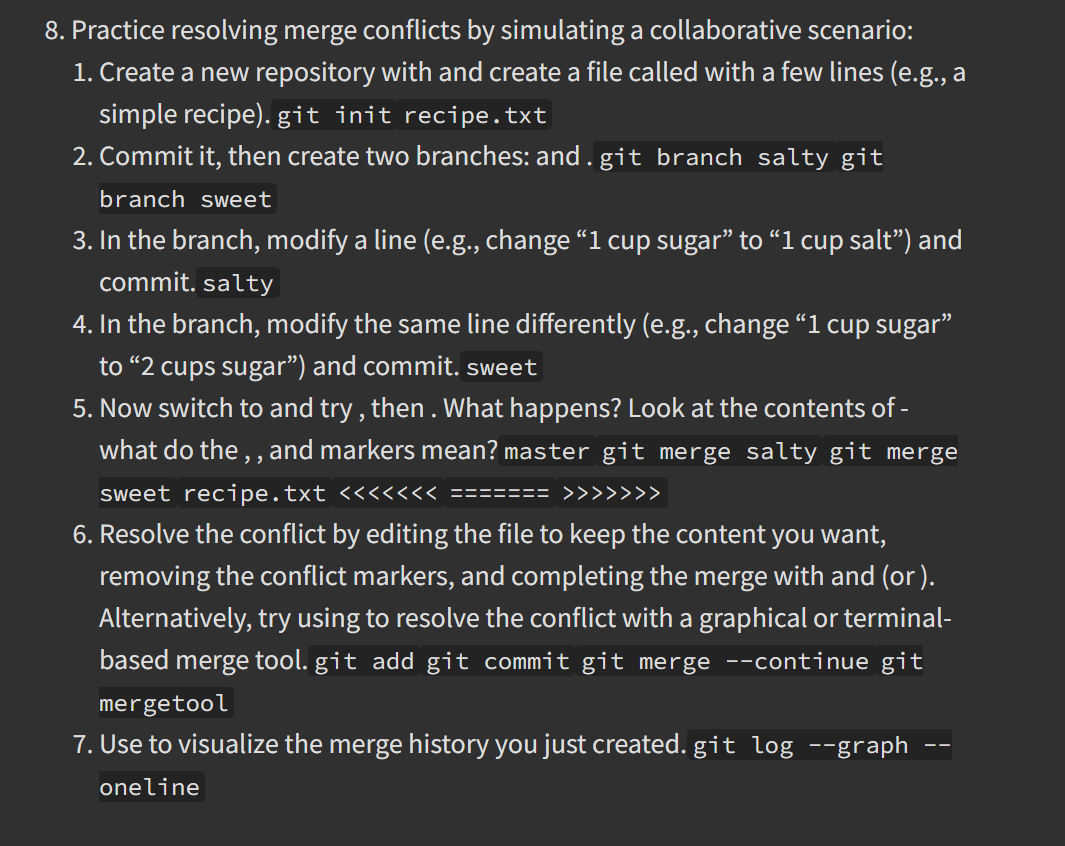
\includegraphics[width=0.9\textwidth]{fig_git8_question.png}
    \caption{Git 第 8 题题目截图}
    \label{fig:git8_question}
\end{figure}

\textbf{作答}：
\begin{lstlisting}[language=bash, caption={制造并解决冲突}]
git init
# recipe.txt 中含 "1 cup sugar" 等行
git add recipe.txt && git commit -m "init recipe"
git branch salty && git branch sweet
git switch salty   # 将 "1 cup sugar" 改为 "1 cup salt" 并提交
git switch sweet   # 将 "1 cup sugar" 改为 "2 cups sugar" 并提交
git switch master
git merge salty
git merge sweet    # 冲突
# 编辑 recipe.txt 保留所需内容，删除冲突标记
git add recipe.txt && git commit   # 或 git merge --continue
git log --graph --oneline
\end{lstlisting}

\textbf{结果}：冲突标记 \texttt{<<<<<<<} 到 \texttt{=======} 之间是当前分支（HEAD）的内容，\texttt{=======} 到 \texttt{>>>>>>>} 之间是待合并分支的内容。解决冲突后的 \texttt{recipe.txt} 内容如下：
\begin{lstlisting}[caption={解决冲突后的 recipe.txt}]
1 cup salt
2 cups sugar
2 cup water
\end{lstlisting}

合并完成后用 \texttt{git log --graph --oneline} 可以看到分叉又合并的提交历史。

\begin{figure}[H]
    \centering
    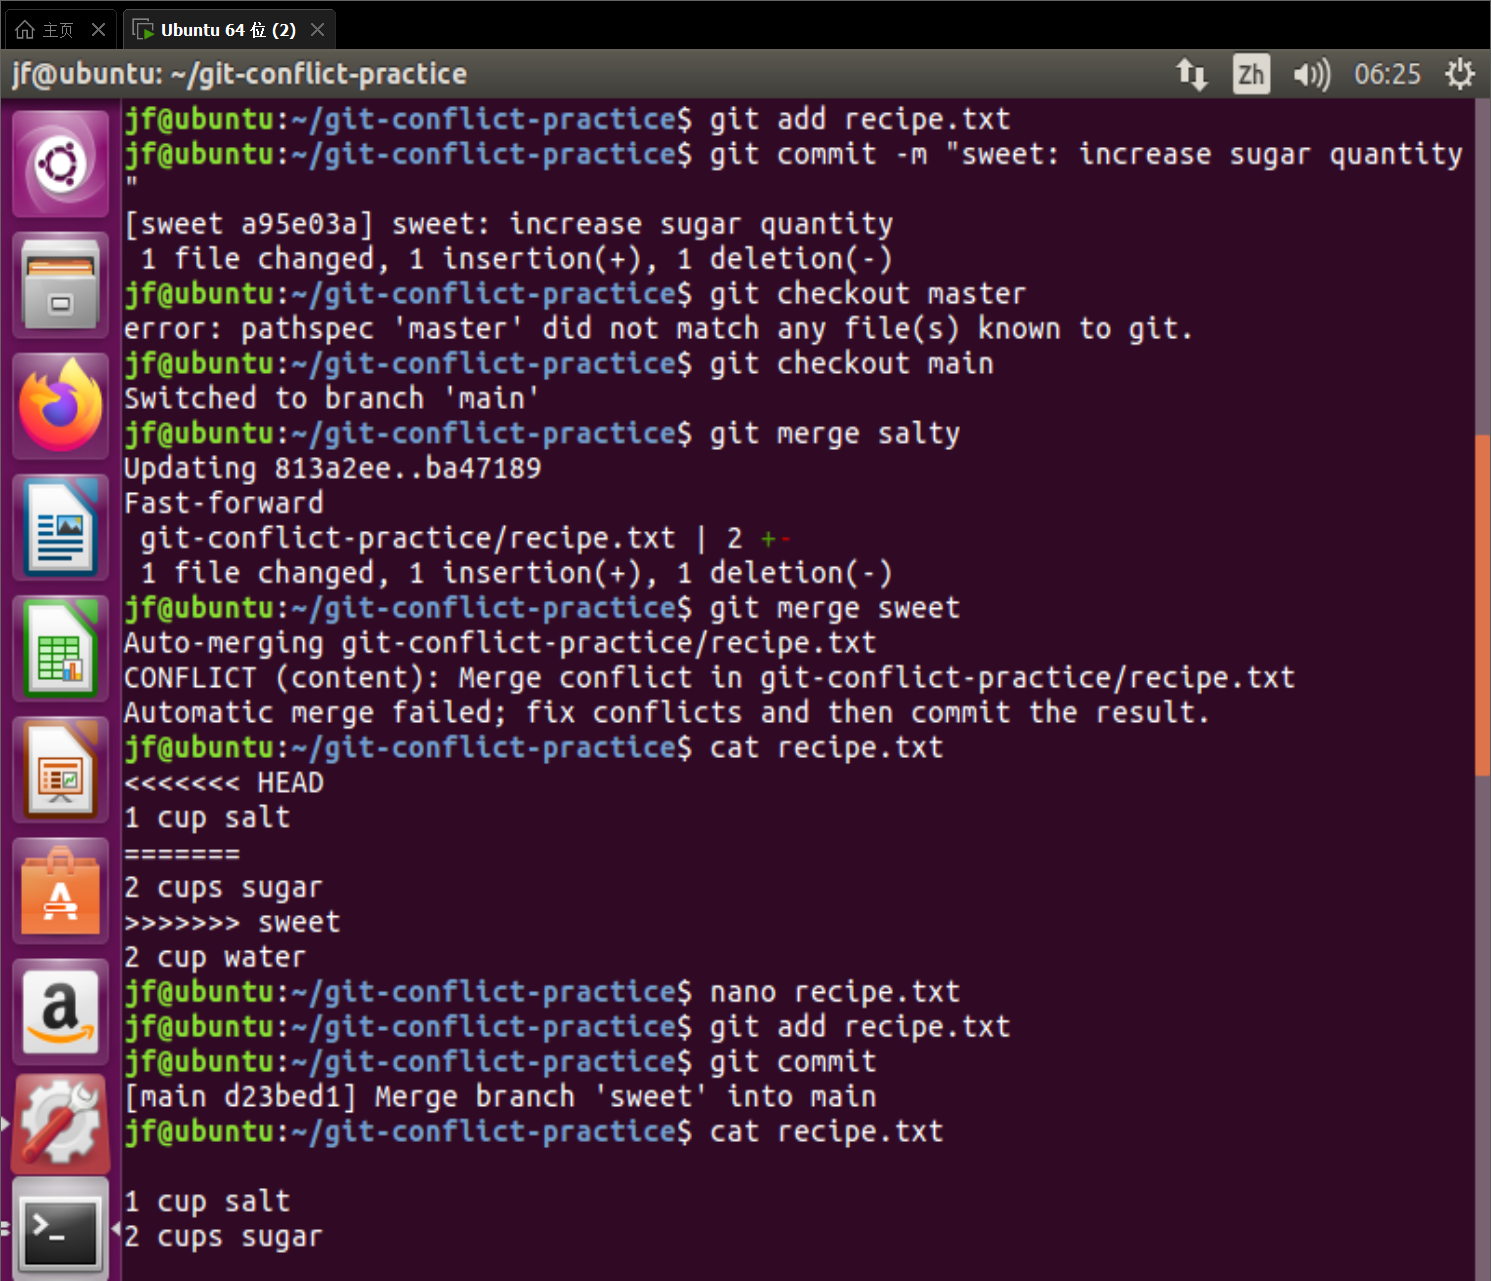
\includegraphics[width=0.9\textwidth]{fig_git8_merge_conflict.png}
    \caption{合并冲突的产生与解决过程}
    \label{fig:git8_merge_conflict}
\end{figure}

\begin{figure}[H]
    \centering
    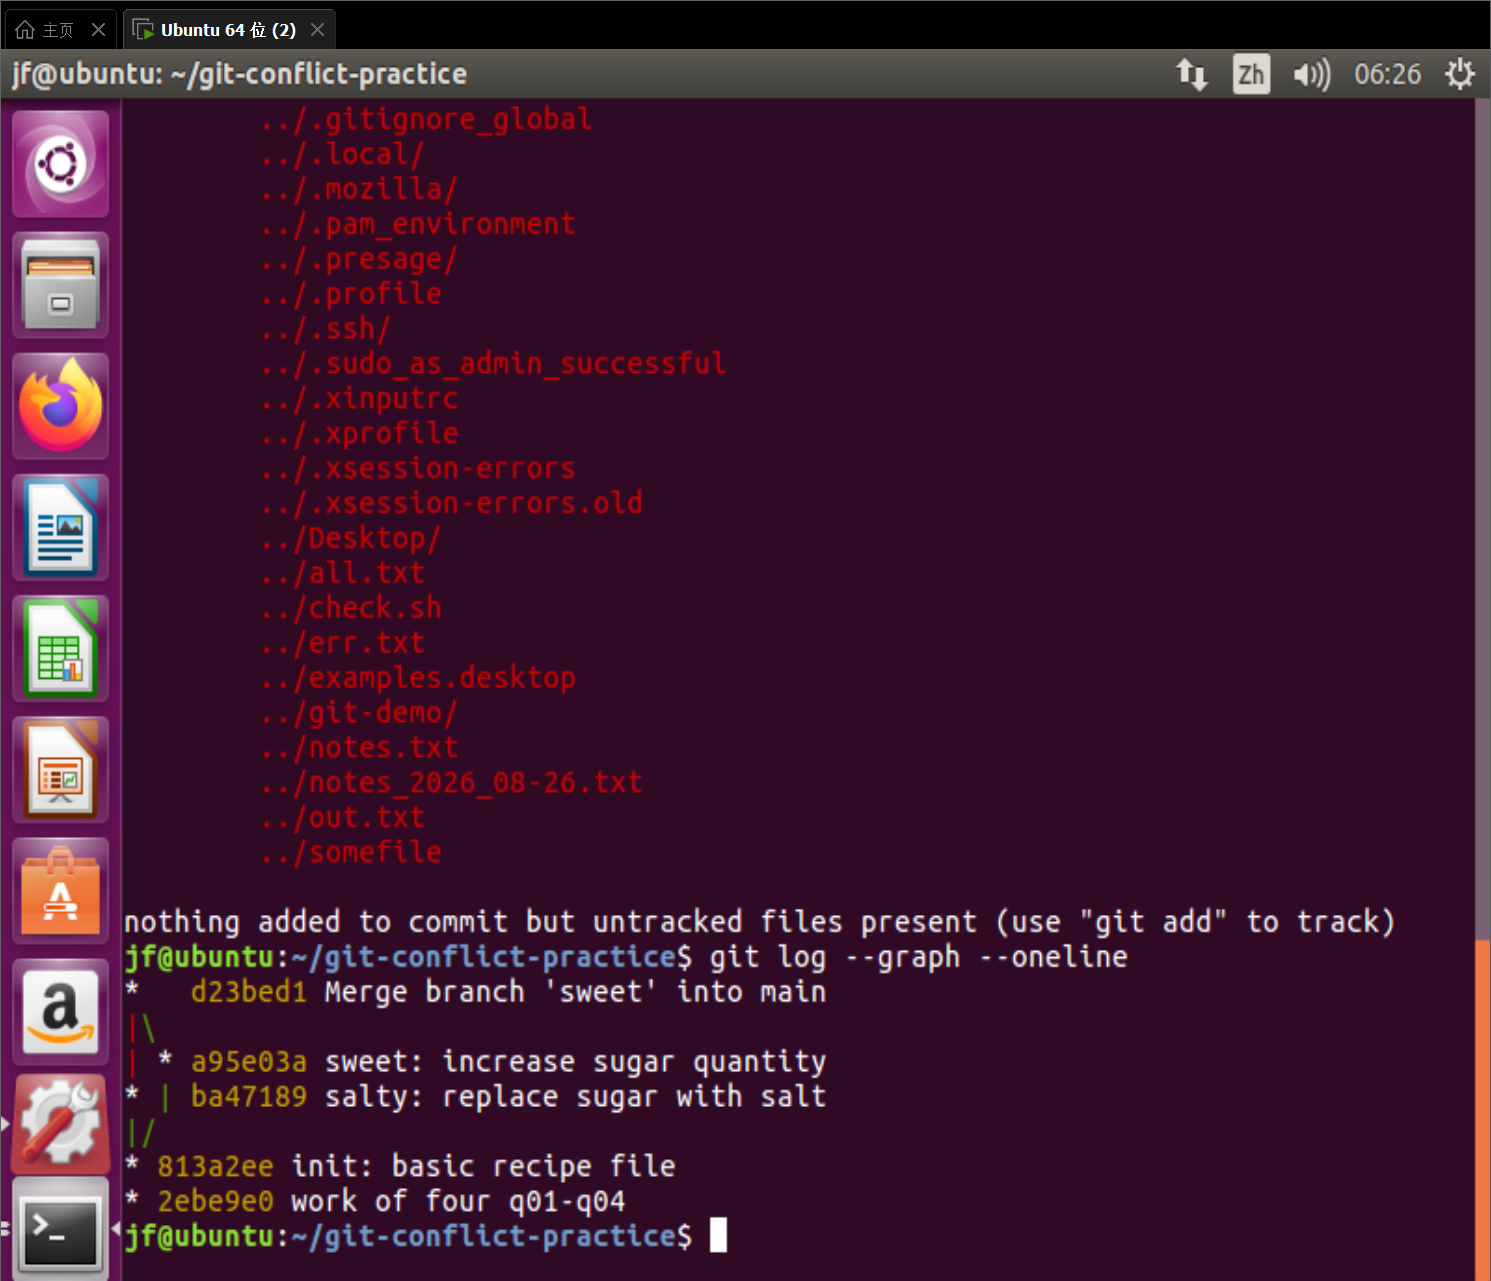
\includegraphics[width=0.9\textwidth]{fig_git8_log.png}
    \caption{git log --graph --oneline 查看合并历史}
    \label{fig:git8_log}
\end{figure}

% ============================================================================
% 3. 解题感悟
% ============================================================================
\section{解题感悟}

\subsection{遇到的问题}

本次实验中遇到的问题主要有：
\begin{enumerate}
    \item \textbf{含空格的文件名处理}：在 q01 复制带空格的 \texttt{notes one.txt} 时，若不使用引号，命令会被拆分为多个参数导致失败；
    \item \textbf{合并冲突}：q03 与课后练习中，两个分支修改同一行导致冲突，需要手工判断保留内容并删除冲突标记；
    \item \textbf{脚本无法直接运行}：写好的 \texttt{check.sh} 直接运行报 Permission denied，原因是缺少可执行权限；
    \item \textbf{标准流混淆}：刚开始分不清 stdout 与 stderr，错误输出和正常输出混在一起。
\end{enumerate}

\subsection{解决过程}

\begin{enumerate}
    \item 对文件名加引号并使用 \texttt{find -exec sh -c} 批量处理，成功保留相对目录结构并处理了空格；
    \item 通过查看 \texttt{<<<<<<< / ======= / >>>>>>>} 标记含义，理解了冲突来源，编辑保留 \texttt{mode=safe} 并添加 \texttt{note=reviewed} 完成合并；
    \item 执行 \texttt{chmod +x} 并对比 \texttt{ls -l} 前后输出，理解了执行权限的意义；
    \item 分别用 \texttt{>} 和 \texttt{2>} 重定向到不同文件，再用 \texttt{2>\&1} 合并，彻底理解了三条标准流。
\end{enumerate}

\subsection{收获与反思}

通过本次实验，我掌握了 Shell 文件系统操作、管道与文本处理、Git 分支与合并冲突的解决、以及 LaTeX 文档构建的基本技能。体会到：
\begin{itemize}
    \item 命令行工具之间通过管道组合能高效完成任务，但要注意数据格式；
    \item Git 的冲突不是错误，而是需要人工决策的合并信号，理解冲突标记是解决冲突的关键；
    \item 养成使用 Git 分步提交、配置忽略文件的好习惯，能有效避免误提交和后期返工。
\end{itemize}

% ============================================================================
% 4. 代码仓库与提交记录
% ============================================================================
\section{代码仓库与提交记录}\label{sec:repo}

按照课程要求，每次课程的报告、练习、代码等均上传到个人 GitHub 账号，保留 commit 记录，并禁止单次全量提交（分步、分主题多次提交）。

\subsection{仓库链接}
\begin{itemize}
    \item GitHub 仓库地址：\url{https://github.com/GJF080117/jf}
    \item 本次实验对应分支：\texttt{main}
\end{itemize}

个人 GitHub 仓库 \texttt{jf} 主页截图如下，可看到按 q01--q04、git-demo、git-conflict-practice 等分目录组织的课程作业，以及各文件的提交记录：

\begin{figure}[H]
    \centering
    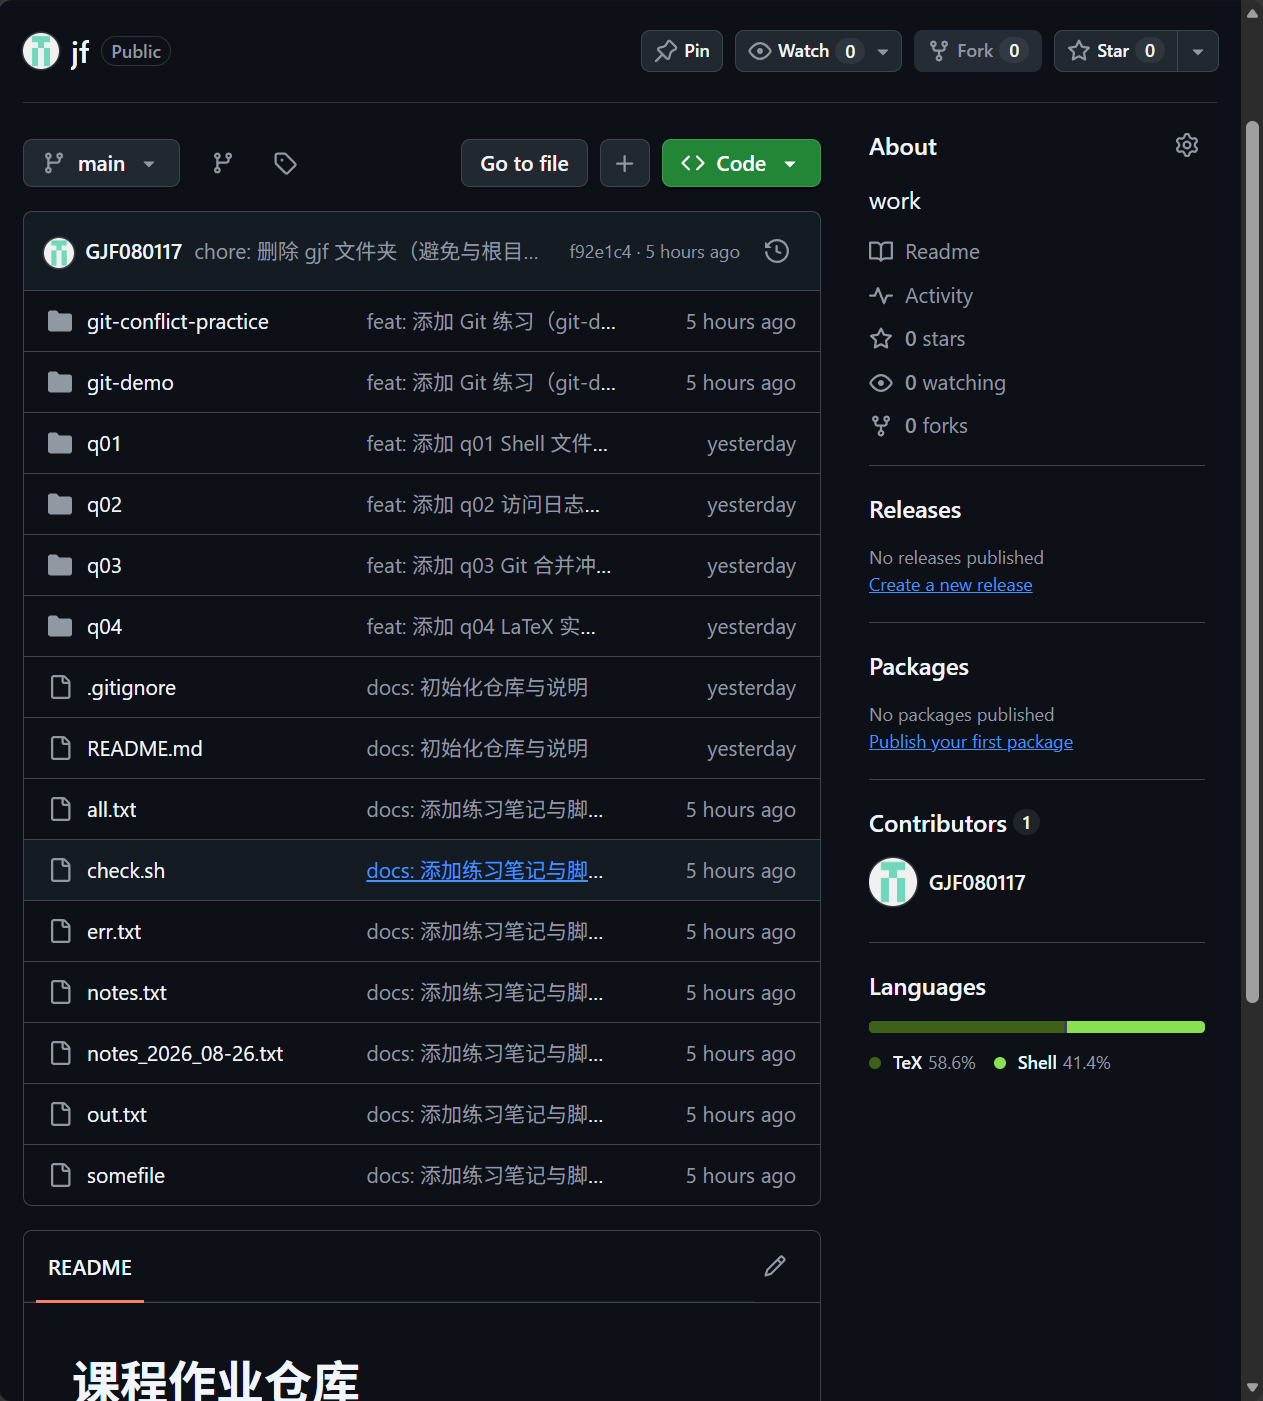
\includegraphics[width=0.9\textwidth]{fig_repo_home.png}
    \caption{GitHub 仓库 jf 主页（文件列表与提交记录）}
    \label{fig:repo_home}
\end{figure}

\subsection{commit 记录}

本次实验的分步提交记录如下（\texttt{git log --oneline}）：

\begin{lstlisting}[caption={jf 仓库提交记录}]
f92e1c4 chore: 删除 gjf 文件夹（避免与根目录 q01-q04 重复）
e2e8b88 feat: 添加 gjf 作业文件夹
790ab3d docs: 添加练习笔记与脚本文件
6d9b53a feat: 添加 Git 练习（git-demo 与 git-conflict-practice）
65e5d75 feat: 添加 q04 LaTeX 实验报告
6de435c feat: 添加 q03 Git 合并冲突实验
c96442f feat: 添加 q02 访问日志统计
223c32d feat: 添加 q01 Shell 文件系统实验
5a2a3e0 docs: 初始化仓库与说明
\end{lstlisting}

GitHub 网页上的 commit 记录截图如下，可清晰看到分步、分主题的多次提交历史：

\begin{figure}[H]
    \centering
    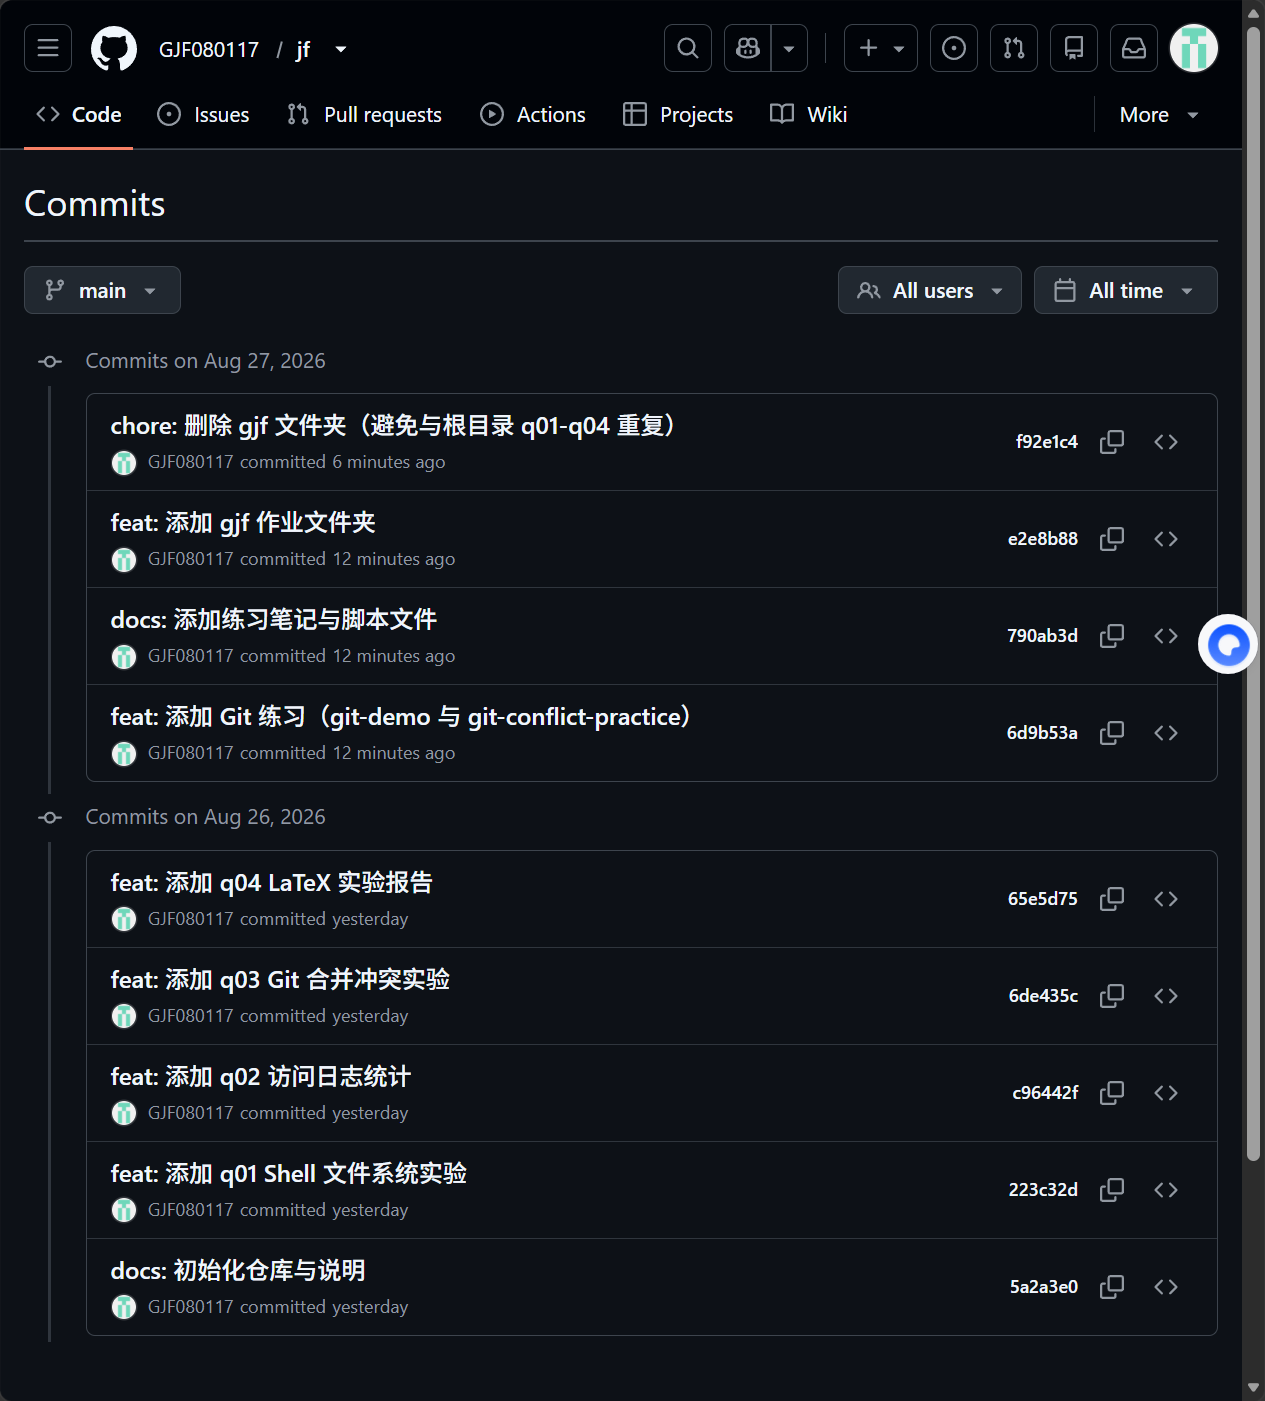
\includegraphics[width=0.85\textwidth]{fig_commit_history.png}
    \caption{GitHub jf 仓库 commit 记录截图}
    \label{fig:commit}
\end{figure}

\subsection{提交说明}

提交采用「先初始化、再按 q01--q04 分题提交、最后补充练习笔记与 Git 练习」的分步策略，每次提交均附有清晰的 commit message，避免单次全量提交，便于助教查看每一道题的完成过程。

% ============================================================================
% 声明
% ============================================================================
\vspace{2em}
\begin{flushright}
    \begin{minipage}{0.55\textwidth}
        \noindent 本人声明：本报告内容为本人独立完成，代码与练习均来自本人实际操作。\\
        \vspace{0.8em}
        \hfill 签名：\underline{\hspace{4em}} \\
        \hfill 日期：\underline{\hspace{4em}}
    \end{minipage}
\end{flushright}

\end{document}
